% !TeX program = pdfLaTeX
\documentclass[12pt]{article}
\usepackage{amsmath}
\usepackage{graphicx,psfrag,epsf}
\usepackage{enumerate}
\usepackage{natbib}
\usepackage{textcomp}
\usepackage[hyphens]{url} % not crucial - just used below for the URL
\usepackage{hyperref}
\providecommand{\tightlist}{%
  \setlength{\itemsep}{0pt}\setlength{\parskip}{0pt}}

%\pdfminorversion=4
% NOTE: To produce blinded version, replace "0" with "1" below.
\newcommand{\blind}{0}

% DON'T change margins - should be 1 inch all around.
\addtolength{\oddsidemargin}{-.5in}%
\addtolength{\evensidemargin}{-.5in}%
\addtolength{\textwidth}{1in}%
\addtolength{\textheight}{1.3in}%
\addtolength{\topmargin}{-.8in}%

%% load any required packages here


\usepackage{color}
\usepackage{fancyvrb}
\newcommand{\VerbBar}{|}
\newcommand{\VERB}{\Verb[commandchars=\\\{\}]}
\DefineVerbatimEnvironment{Highlighting}{Verbatim}{commandchars=\\\{\}}
% Add ',fontsize=\small' for more characters per line
\usepackage{framed}
\definecolor{shadecolor}{RGB}{248,248,248}
\newenvironment{Shaded}{\begin{snugshade}}{\end{snugshade}}
\newcommand{\AlertTok}[1]{\textcolor[rgb]{0.94,0.16,0.16}{#1}}
\newcommand{\AnnotationTok}[1]{\textcolor[rgb]{0.56,0.35,0.01}{\textbf{\textit{#1}}}}
\newcommand{\AttributeTok}[1]{\textcolor[rgb]{0.77,0.63,0.00}{#1}}
\newcommand{\BaseNTok}[1]{\textcolor[rgb]{0.00,0.00,0.81}{#1}}
\newcommand{\BuiltInTok}[1]{#1}
\newcommand{\CharTok}[1]{\textcolor[rgb]{0.31,0.60,0.02}{#1}}
\newcommand{\CommentTok}[1]{\textcolor[rgb]{0.56,0.35,0.01}{\textit{#1}}}
\newcommand{\CommentVarTok}[1]{\textcolor[rgb]{0.56,0.35,0.01}{\textbf{\textit{#1}}}}
\newcommand{\ConstantTok}[1]{\textcolor[rgb]{0.00,0.00,0.00}{#1}}
\newcommand{\ControlFlowTok}[1]{\textcolor[rgb]{0.13,0.29,0.53}{\textbf{#1}}}
\newcommand{\DataTypeTok}[1]{\textcolor[rgb]{0.13,0.29,0.53}{#1}}
\newcommand{\DecValTok}[1]{\textcolor[rgb]{0.00,0.00,0.81}{#1}}
\newcommand{\DocumentationTok}[1]{\textcolor[rgb]{0.56,0.35,0.01}{\textbf{\textit{#1}}}}
\newcommand{\ErrorTok}[1]{\textcolor[rgb]{0.64,0.00,0.00}{\textbf{#1}}}
\newcommand{\ExtensionTok}[1]{#1}
\newcommand{\FloatTok}[1]{\textcolor[rgb]{0.00,0.00,0.81}{#1}}
\newcommand{\FunctionTok}[1]{\textcolor[rgb]{0.00,0.00,0.00}{#1}}
\newcommand{\ImportTok}[1]{#1}
\newcommand{\InformationTok}[1]{\textcolor[rgb]{0.56,0.35,0.01}{\textbf{\textit{#1}}}}
\newcommand{\KeywordTok}[1]{\textcolor[rgb]{0.13,0.29,0.53}{\textbf{#1}}}
\newcommand{\NormalTok}[1]{#1}
\newcommand{\OperatorTok}[1]{\textcolor[rgb]{0.81,0.36,0.00}{\textbf{#1}}}
\newcommand{\OtherTok}[1]{\textcolor[rgb]{0.56,0.35,0.01}{#1}}
\newcommand{\PreprocessorTok}[1]{\textcolor[rgb]{0.56,0.35,0.01}{\textit{#1}}}
\newcommand{\RegionMarkerTok}[1]{#1}
\newcommand{\SpecialCharTok}[1]{\textcolor[rgb]{0.00,0.00,0.00}{#1}}
\newcommand{\SpecialStringTok}[1]{\textcolor[rgb]{0.31,0.60,0.02}{#1}}
\newcommand{\StringTok}[1]{\textcolor[rgb]{0.31,0.60,0.02}{#1}}
\newcommand{\VariableTok}[1]{\textcolor[rgb]{0.00,0.00,0.00}{#1}}
\newcommand{\VerbatimStringTok}[1]{\textcolor[rgb]{0.31,0.60,0.02}{#1}}
\newcommand{\WarningTok}[1]{\textcolor[rgb]{0.56,0.35,0.01}{\textbf{\textit{#1}}}}

% Pandoc citation processing


\begin{document}


\def\spacingset#1{\renewcommand{\baselinestretch}%
{#1}\small\normalsize} \spacingset{1}


%%%%%%%%%%%%%%%%%%%%%%%%%%%%%%%%%%%%%%%%%%%%%%%%%%%%%%%%%%%%%%%%%%%%%%%%%%%%%%

\if0\blind
{
  \title{\bf Analyzing centralitty measures for a sexual network of gonorrhea transmission}

  \author{
        J Steven Raquel \\
    Department of Statistics, University of California, Irvine\\
      }
  \maketitle
} \fi

\if1\blind
{
  \bigskip
  \bigskip
  \bigskip
  \begin{center}
    {\LARGE\bf Analyzing centralitty measures for a sexual network of gonorrhea transmission}
  \end{center}
  \medskip
} \fi

\bigskip
\begin{abstract}

\end{abstract}

\noindent%
{\it Keywords:} social network analysis, sexually transmitted diseases, epidemiology, centrality, clustering
\vfill

\newpage
\spacingset{1.45} % DON'T change the spacing!

\hypertarget{introduction}{%
\section{Introduction}\label{introduction}}

Contact tracing for sexually transmitted diseases (STDs) such as gonorrhea, chlamydia, syphilis etc. is a persistent epidemiological problem, as it depends on individuals getting routinely tested as well as informing their sexual partners of their positive diagnosis should they receive one. Compounding this with the fact that many of these positive cases can be symptomless but still contagious creates a serious issue. Gonorrhea in particular is a disease that can be asymptomatic in both men and women who have it, that can go so far as causing infertility or lead to a life-threatening condition.

This dataset, constructed in the form of an adjacency matrix, contains 89 nodes, one of which is the ``event'' of attending a bar (i.e.~when a node has a tie with this bar node, it means they attend the bar). Two of these nodes (denoted by \texttt{x} and \texttt{x2}) are missing information about their gender which is otherwise indicated by an \texttt{m} or \texttt{f} in the label of the respective node, followed by a number with which to differentiate them.

The network is directed, and the criteria for some node \(i\) to have a tie with some other node \(j\) must be that that \(i\)th node named node \(j\) as a prior sexual partner.

The data was collected from a series of adjacent aboriginal communities located in the province of Alberta, Canada, where public health officials took note of a local gonorrhea outbreak and confirmed that attendance at a local bar in one such community was associated with infection (De 2003).

\hypertarget{methods}{%
\section{Methods}\label{methods}}

\begin{Shaded}
\begin{Highlighting}[]
\FunctionTok{par}\NormalTok{(}\AttributeTok{mfrow =} \FunctionTok{c}\NormalTok{(}\DecValTok{1}\NormalTok{,}\DecValTok{1}\NormalTok{))}
\FunctionTok{set.seed}\NormalTok{(}\DecValTok{10}\NormalTok{)}
\NormalTok{org\_coord }\OtherTok{\textless{}{-}} 
  \FunctionTok{gplot}\NormalTok{(gonnet, }\AttributeTok{vertex.col =}\NormalTok{ gonnet\_df}\SpecialCharTok{$}\NormalTok{col,}
      \AttributeTok{vertex.sides =}\NormalTok{ gonnet\_df}\SpecialCharTok{$}\NormalTok{gender\_lty,}
      \AttributeTok{displaylabels =}\NormalTok{ T, }\AttributeTok{label.cex =} \FloatTok{0.6}\NormalTok{,}
      \AttributeTok{boxed.labels =}\NormalTok{ F, }\AttributeTok{pad =} \DecValTok{2}\NormalTok{, }\AttributeTok{usearrows =}\NormalTok{ T,}
      \AttributeTok{vertex.cex =} \FloatTok{1.25}\NormalTok{)}
\CommentTok{\# legend for gender}
\FunctionTok{legend}\NormalTok{(}\StringTok{"topleft"}\NormalTok{,}
       \AttributeTok{legend =} \FunctionTok{c}\NormalTok{(}\StringTok{"yes"}\NormalTok{, }\StringTok{"no"}\NormalTok{),}
       \AttributeTok{col =} \FunctionTok{c}\NormalTok{(}\StringTok{"tomato1"}\NormalTok{, }\StringTok{"grey"}\NormalTok{),}
       \AttributeTok{fill =}\NormalTok{ F, }\AttributeTok{border =} \StringTok{"white"}\NormalTok{, }\AttributeTok{pch =} \DecValTok{19}\NormalTok{,}
       \AttributeTok{title =} \StringTok{"Bar Attendance"}\NormalTok{, }\AttributeTok{bty =} \StringTok{"n"}\NormalTok{)}
\FunctionTok{legend}\NormalTok{(}\StringTok{"topright"}\NormalTok{,}
       \AttributeTok{legend =} \FunctionTok{c}\NormalTok{(}\StringTok{"m"}\NormalTok{, }\StringTok{"f"}\NormalTok{),}
       \AttributeTok{col =} \FunctionTok{c}\NormalTok{(}\StringTok{"black"}\NormalTok{),}
       \AttributeTok{fill =}\NormalTok{ F, }\AttributeTok{border =} \StringTok{"white"}\NormalTok{, }\AttributeTok{pch =} \FunctionTok{c}\NormalTok{(}\DecValTok{0}\NormalTok{, }\DecValTok{2}\NormalTok{),}
       \AttributeTok{title =} \StringTok{"Gender"}\NormalTok{, }\AttributeTok{bty =} \StringTok{"n"}\NormalTok{)}
\end{Highlighting}
\end{Shaded}

\begin{figure}
\centering
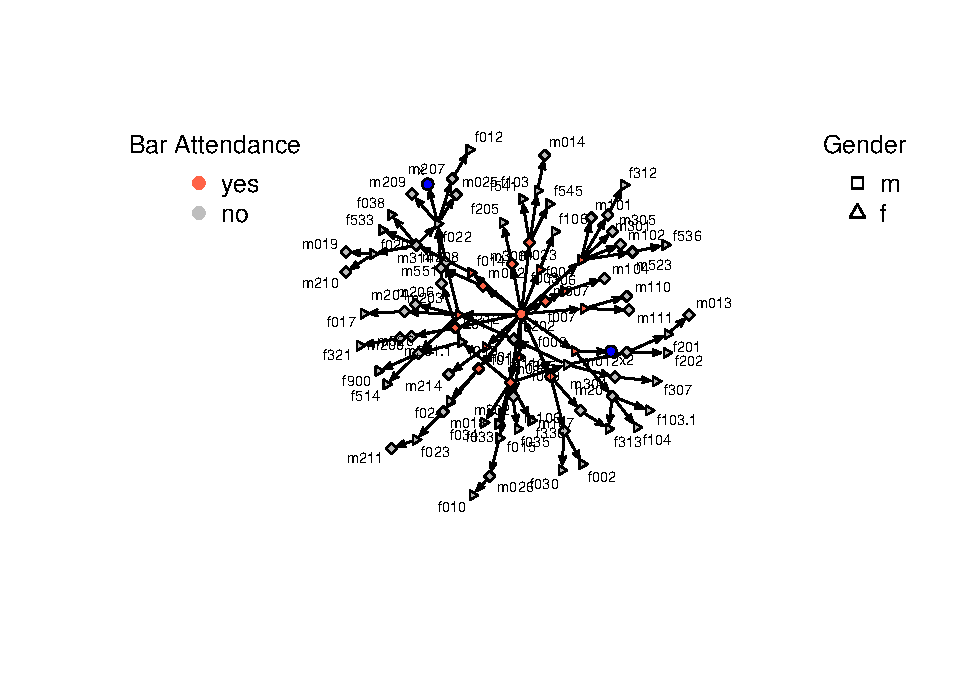
\includegraphics{JStevenRaquel-paper_files/figure-latex/sociogram-1.pdf}
\caption{\label{fig:sociogram}Sociogram of the gonorrhea network.}
\end{figure}

\begin{Shaded}
\begin{Highlighting}[]
\CommentTok{\# legend for bar attendance}
\end{Highlighting}
\end{Shaded}

Looking at this initial sociogram, where the bar node is firmly in the center, we see that it has outgoing connections to 17 nodes, which themselves have connections to at least one other node in the rest of the network.

The majority of ties are between individuals of the opposite sex, e.g.~male-to-female or female-to-male, but there are a minority of instances where individuals have a tie to individuals of the same sex, e.g.~m112 has ties with both m106 and m107, who both in turn have ties to at least one female node.

The node m010 is also unique in that it happens to have outgoing ties to one female node (f024) and one male node (m018), the latter of which in turn has a tie with a female node (f023). The idea of men who have sex with men (MSM) or women who have sex with women (WSW) acting as bridging nodes between otherwise disparate sexual networks was something considered in the exploratory analysis but there just wasn't enough data to delve deeper into this subject.

The first approach in the analysis was to look at the \emph{centrality measures} of each of the nodes.

\hypertarget{centrality-measures}{%
\subsection{Centrality Measures}\label{centrality-measures}}

\begin{verbatim}
##              outdegree   indegree betweenness eigenvector
## outdegree    1.0000000 -0.1970015  0.40612528  0.79067530
## indegree    -0.1970015  1.0000000  0.52061632 -0.37578288
## betweenness  0.4061253  0.5206163  1.00000000 -0.05333083
## eigenvector  0.7906753 -0.3757829 -0.05333083  1.00000000
\end{verbatim}

\begin{verbatim}
##              outdegree   indegree betweenness eigenvector
## outdegree    1.0000000  1.0000000   0.9543577  -0.8172166
## indegree     1.0000000  1.0000000   0.9543577  -0.8172166
## betweenness  0.9543577  0.9543577   1.0000000  -0.8603699
## eigenvector -0.8172166 -0.8172166  -0.8603699   1.0000000
\end{verbatim}

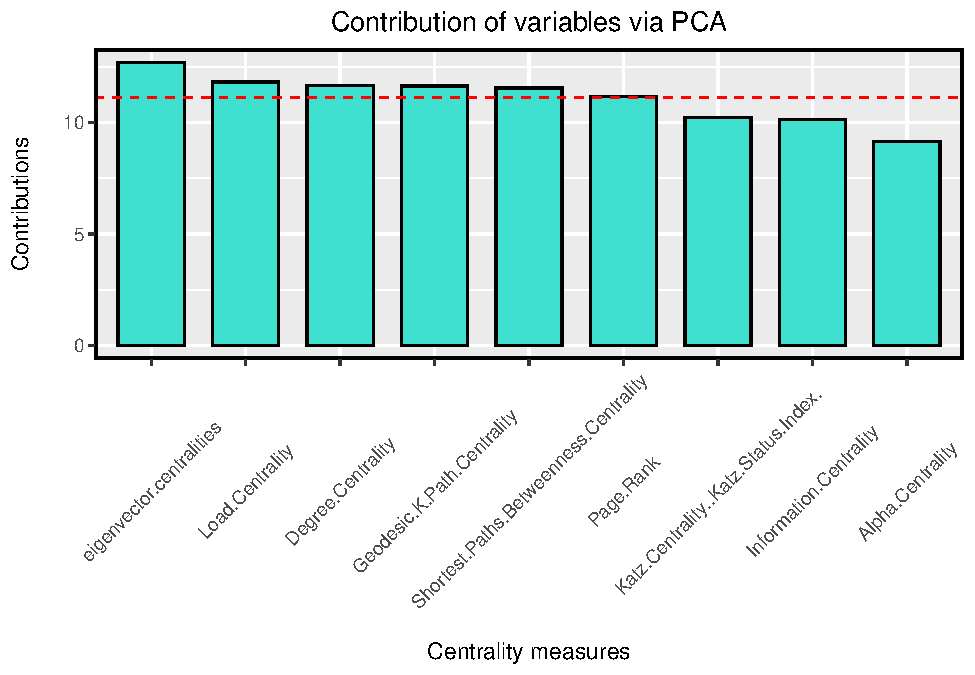
\includegraphics{JStevenRaquel-paper_files/figure-latex/centralities_more-1.pdf}

According to Borgatti and Everett (2006), \emph{centrality} is a summary index of a node's position in a graph, based on sums or averages of one of several things: 1) the number of edges the node has, 2) the length of the paths that end up at the node, or 3) the proportion of paths that contain the node inside of it (not as an endpoint).

Different measures of centrality depend on functions of one of these aspects and communicate different things about a node, depending on the algorithm for the centrality measure. Among the centrality measures used in this analysis were that of \emph{degree centrality}, \emph{eigenvector centrality}, \emph{load centrality}, and \emph{information centrality}.

\hypertarget{degree-centrality}{%
\subsubsection{Degree Centrality}\label{degree-centrality}}

Degree centrality can be measured in multiple ways; the first is \emph{indegree} which is a count of the number of incoming ties that a node has. The second is \emph{outdegree} which conversely is the count of the number of outgoing ties that a node has.

The vast majority of nodes in the directed network have an indegree of 1, i.e.~only one individual nominated that person as a sexual partner when interviewed. The outdegree was \emph{at least} 1 for most nodes in the network, but could be zero for nodes on the very outside of the network who did not name any sexual partners.

The overall degree of a node can be taken as the total amount of ties a node has, either incoming or outgoing, but in the case of an undirected graph, these are one and the same.

\hypertarget{outdegree-centrality}{%
\paragraph{Outdegree Centrality}\label{outdegree-centrality}}

\begin{Shaded}
\begin{Highlighting}[]
\NormalTok{gonnet\_df2 }\OtherTok{\textless{}{-}} \FunctionTok{cbind}\NormalTok{(gonnet\_df, cen) }\SpecialCharTok{\%\textgreater{}\%} \FunctionTok{select}\NormalTok{(}\SpecialCharTok{{-}}\NormalTok{id)}

\CommentTok{\# boxplot comparing outdegree}
\NormalTok{outdegree\_gender }\OtherTok{\textless{}{-}}\NormalTok{ gonnet\_df2 }\SpecialCharTok{\%\textgreater{}\%} 
  \FunctionTok{select}\NormalTok{(nodes, gender, outdegree) }\SpecialCharTok{\%\textgreater{}\%} 
  \FunctionTok{drop\_na}\NormalTok{()}

\CommentTok{\# boxplot of outdegree by gender}
\FunctionTok{ggplot}\NormalTok{(outdegree\_gender, }\FunctionTok{aes}\NormalTok{(}\AttributeTok{x=}\NormalTok{gender, }\AttributeTok{y=}\NormalTok{outdegree)) }\SpecialCharTok{+} 
  \FunctionTok{geom\_boxplot}\NormalTok{()}
\end{Highlighting}
\end{Shaded}

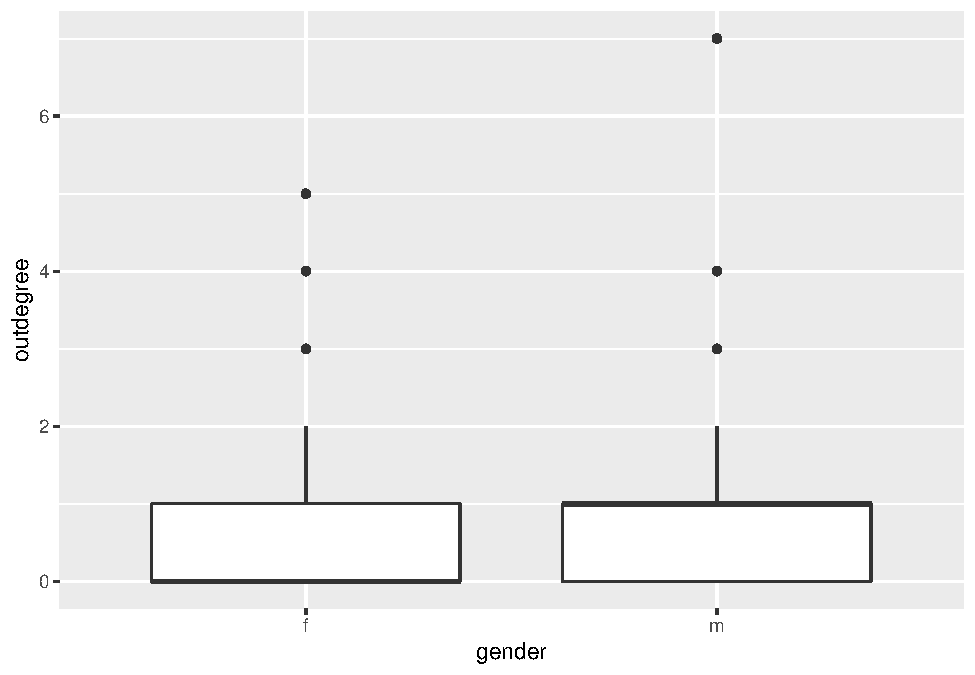
\includegraphics{JStevenRaquel-paper_files/figure-latex/male-female-outdegree-1.pdf}

\begin{Shaded}
\begin{Highlighting}[]
\CommentTok{\# average outdegree overall}
\NormalTok{gonnet\_df2}\SpecialCharTok{$}\NormalTok{outdegree }\SpecialCharTok{\%\textgreater{}\%} \FunctionTok{mean}\NormalTok{()}
\end{Highlighting}
\end{Shaded}

\begin{verbatim}
## [1] 1.044944
\end{verbatim}

\begin{Shaded}
\begin{Highlighting}[]
\CommentTok{\# average outdegree among males in network, overall}
\NormalTok{outdegree\_m }\OtherTok{\textless{}{-}}\NormalTok{ gonnet\_df2 }\SpecialCharTok{\%\textgreater{}\%}
  \FunctionTok{select}\NormalTok{(nodes, gender, outdegree) }\SpecialCharTok{\%\textgreater{}\%}
  \FunctionTok{filter}\NormalTok{(gender }\SpecialCharTok{==} \StringTok{"m"}\NormalTok{) }\SpecialCharTok{\%\textgreater{}\%}
  \FunctionTok{select}\NormalTok{(outdegree) }\SpecialCharTok{\%\textgreater{}\%} 
  \FunctionTok{unlist}\NormalTok{()}
\NormalTok{outdegree\_m }\SpecialCharTok{\%\textgreater{}\%} \FunctionTok{mean}\NormalTok{()}
\end{Highlighting}
\end{Shaded}

\begin{verbatim}
## [1] 0.9767442
\end{verbatim}

\begin{Shaded}
\begin{Highlighting}[]
\NormalTok{outdegree\_m }\SpecialCharTok{\%\textgreater{}\%} \FunctionTok{median}\NormalTok{()}
\end{Highlighting}
\end{Shaded}

\begin{verbatim}
## [1] 1
\end{verbatim}

\begin{Shaded}
\begin{Highlighting}[]
\CommentTok{\# male outdegree that excludes nodes with zero outdegree}
\NormalTok{gonnet\_df2 }\SpecialCharTok{\%\textgreater{}\%}
  \FunctionTok{select}\NormalTok{(nodes, gender, outdegree) }\SpecialCharTok{\%\textgreater{}\%}
  \FunctionTok{filter}\NormalTok{(gender }\SpecialCharTok{==} \StringTok{"m"} \SpecialCharTok{\&}\NormalTok{ outdegree }\SpecialCharTok{!=} \DecValTok{0}\NormalTok{) }\SpecialCharTok{\%\textgreater{}\%}
  \FunctionTok{select}\NormalTok{(outdegree) }\SpecialCharTok{\%\textgreater{}\%}
  \FunctionTok{unlist}\NormalTok{() }\SpecialCharTok{\%\textgreater{}\%} \FunctionTok{mean}\NormalTok{()}
\end{Highlighting}
\end{Shaded}

\begin{verbatim}
## [1] 1.826087
\end{verbatim}

\begin{Shaded}
\begin{Highlighting}[]
\CommentTok{\# average outdegree among females}
\NormalTok{outdegree\_f }\OtherTok{\textless{}{-}}\NormalTok{ gonnet\_df2 }\SpecialCharTok{\%\textgreater{}\%} 
  \FunctionTok{select}\NormalTok{(nodes, gender, outdegree) }\SpecialCharTok{\%\textgreater{}\%}
  \FunctionTok{filter}\NormalTok{(gender }\SpecialCharTok{==} \StringTok{"f"}\NormalTok{) }\SpecialCharTok{\%\textgreater{}\%} 
  \FunctionTok{select}\NormalTok{(outdegree) }\SpecialCharTok{\%\textgreater{}\%}
  \FunctionTok{unlist}\NormalTok{()}
\NormalTok{outdegree\_f }\SpecialCharTok{\%\textgreater{}\%} \FunctionTok{mean}\NormalTok{()}
\end{Highlighting}
\end{Shaded}

\begin{verbatim}
## [1] 0.7906977
\end{verbatim}

\begin{Shaded}
\begin{Highlighting}[]
\NormalTok{outdegree\_f }\SpecialCharTok{\%\textgreater{}\%} \FunctionTok{median}\NormalTok{()}
\end{Highlighting}
\end{Shaded}

\begin{verbatim}
## [1] 0
\end{verbatim}

\begin{Shaded}
\begin{Highlighting}[]
\CommentTok{\# female outdegree that excludes nodes with zero outdegree}
\NormalTok{gonnet\_df2 }\SpecialCharTok{\%\textgreater{}\%}
  \FunctionTok{select}\NormalTok{(nodes, gender, outdegree) }\SpecialCharTok{\%\textgreater{}\%}
  \FunctionTok{filter}\NormalTok{(gender }\SpecialCharTok{==} \StringTok{"f"} \SpecialCharTok{\&}\NormalTok{ outdegree }\SpecialCharTok{!=} \DecValTok{0}\NormalTok{) }\SpecialCharTok{\%\textgreater{}\%}
  \FunctionTok{select}\NormalTok{(outdegree) }\SpecialCharTok{\%\textgreater{}\%}
  \FunctionTok{unlist}\NormalTok{() }\SpecialCharTok{\%\textgreater{}\%} \FunctionTok{mean}\NormalTok{()}
\end{Highlighting}
\end{Shaded}

\begin{verbatim}
## [1] 2
\end{verbatim}

The analysis gave that the overall average outdegree for the directed graph is approximately 1, implying that on average individuals named one sexual partner. It's important to note that many outer edges have an outdegree of 0, which skews down the mean calculation somewhat.

The implication of this observation is two-fold. For one, rather than most individuals in the network having many sexual partners, the implication of how outdegree is distributed in this network is that most individuals have as few as one, but there is a minority of individuals (of both genders) who named more.

\hypertarget{behavioral-considerations}{%
\paragraph{Behavioral Considerations}\label{behavioral-considerations}}

There are some behavioral considerations taken into account when considering this data. The information regarding past sexual partners is entirely self-nominated on the part of the individual who represents the node in the graph, and as such, it's subject to an individual possibly withholding information, for a number of reasons.

There is a social stigma attached to promiscuity (having a high number of sexual partners), as well as living with an STD, so it's important to note that the data may be skewed by dishonesty on the part of the individuals comprising the dataset. For example, a person who receives a positive test result for a sexually transmitted disease may refrain from naming \emph{all} of their recent sexual partners, either to avoid having to communicate the uncomfortable truth of either having contracted or transmitted a disease, or to avoid judgment for divulging what may be perceived as a high number of sexual partners. Societal attitudes towards sex and sexual health both in a Western context and also in an indigenous/Aboriginal context can and should be kept in mind when drawing conclusions from this data.

\begin{verbatim}
## Levene's Test for Homogeneity of Variance (center = median)
##       Df F value Pr(>F)
## group  1  0.2092 0.6486
##       84
\end{verbatim}

\begin{Shaded}
\begin{Highlighting}[]
\CommentTok{\# Student\textquotesingle{}s t{-}test comparing the mean outdegree of men and women}
\CommentTok{\# H0: mu\_x {-} mu\_y = 0}
\FunctionTok{t.test}\NormalTok{(}\AttributeTok{x =}\NormalTok{ outdegree\_m, }
       \AttributeTok{y =}\NormalTok{ outdegree\_f,}
       \AttributeTok{var.equal =}\NormalTok{ T, }\AttributeTok{alternative =} \StringTok{"two.sided"}\NormalTok{)}
\end{Highlighting}
\end{Shaded}

\begin{verbatim}
## 
##  Two Sample t-test
## 
## data:  outdegree_m and outdegree_f
## t = 0.6411, df = 84, p-value = 0.5232
## alternative hypothesis: true difference in means is not equal to 0
## 95 percent confidence interval:
##  -0.3910458  0.7631389
## sample estimates:
## mean of x mean of y 
## 0.9767442 0.7906977
\end{verbatim}

\begin{Shaded}
\begin{Highlighting}[]
\CommentTok{\# p{-}value = 0.5232 \textgreater{} 0.05, we fail to reject H0}
\end{Highlighting}
\end{Shaded}

\hypertarget{eigenvector-centrality}{%
\subsubsection{Eigenvector Centrality}\label{eigenvector-centrality}}

Eigenvector centrality is calculated both as a function of a node's degree but also as a function of the degree of the nodes it is connected to. In other words, a node with a high eigenvector centrality is well-connected to nodes that are themselves well-connected.

\hypertarget{load-centrality}{%
\subsubsection{Load Centrality}\label{load-centrality}}

\hypertarget{information-centrality}{%
\subsubsection{Information Centrality}\label{information-centrality}}

\begin{Shaded}
\begin{Highlighting}[]
\CommentTok{\# boxplot comparing distribution of outdegree between bar (not){-}attended}
\FunctionTok{ggplot}\NormalTok{(gonnet\_df2 }\SpecialCharTok{\%\textgreater{}\%} \FunctionTok{filter}\NormalTok{(}\SpecialCharTok{!}\NormalTok{(nodes }\SpecialCharTok{\%in\%} \FunctionTok{c}\NormalTok{(}\StringTok{"b"}\NormalTok{, }\StringTok{"x"}\NormalTok{, }\StringTok{"x2"}\NormalTok{))), }
       \FunctionTok{aes}\NormalTok{(}\AttributeTok{x =}\NormalTok{ attended\_bar, outdegree)) }\SpecialCharTok{+} 
  \FunctionTok{geom\_boxplot}\NormalTok{() }\SpecialCharTok{+} \FunctionTok{theme\_bw}\NormalTok{()}
\end{Highlighting}
\end{Shaded}

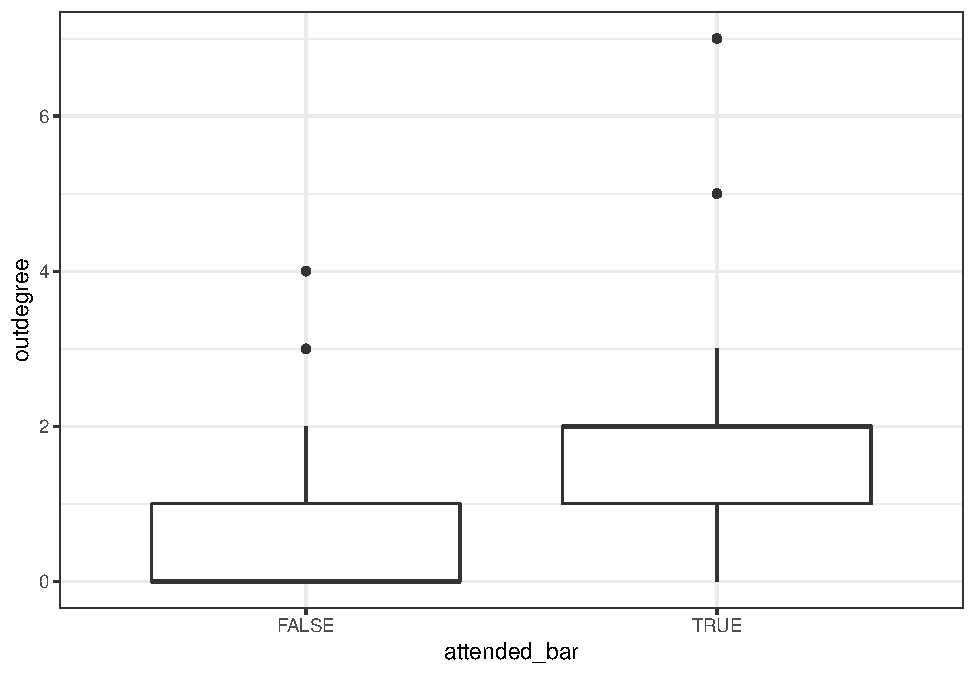
\includegraphics{JStevenRaquel-paper_files/figure-latex/bar-attendance-outdegree-1.pdf}

\begin{Shaded}
\begin{Highlighting}[]
\CommentTok{\# average outdegree among bar attendees}
\NormalTok{outdegree\_bar }\OtherTok{\textless{}{-}}\NormalTok{ gonnet\_df2 }\SpecialCharTok{\%\textgreater{}\%} 
  \FunctionTok{select}\NormalTok{(nodes, attended\_bar, outdegree) }\SpecialCharTok{\%\textgreater{}\%}
  \FunctionTok{filter}\NormalTok{(}\SpecialCharTok{!}\NormalTok{(nodes }\SpecialCharTok{\%in\%} \FunctionTok{c}\NormalTok{(}\StringTok{"b"}\NormalTok{, }\StringTok{"x2"}\NormalTok{, }\StringTok{"x"}\NormalTok{))) }\SpecialCharTok{\%\textgreater{}\%}
  \FunctionTok{filter}\NormalTok{(attended\_bar }\SpecialCharTok{==} \ConstantTok{TRUE}\NormalTok{)}

\CommentTok{\# average outdegree among non{-}bar attendees}
\NormalTok{outdegree\_nobar }\OtherTok{\textless{}{-}}\NormalTok{ gonnet\_df2 }\SpecialCharTok{\%\textgreater{}\%} 
  \FunctionTok{select}\NormalTok{(nodes, attended\_bar, outdegree) }\SpecialCharTok{\%\textgreater{}\%}
  \FunctionTok{filter}\NormalTok{(}\SpecialCharTok{!}\NormalTok{(nodes }\SpecialCharTok{\%in\%} \FunctionTok{c}\NormalTok{(}\StringTok{"b"}\NormalTok{, }\StringTok{"x2"}\NormalTok{, }\StringTok{"x"}\NormalTok{))) }\SpecialCharTok{\%\textgreater{}\%}
  \FunctionTok{filter}\NormalTok{(attended\_bar }\SpecialCharTok{==} \ConstantTok{FALSE}\NormalTok{)}

\CommentTok{\# sample sizes are unequal, so we cannot assume equal variance}
\CommentTok{\# try two{-}sided Welch\textquotesingle{}s t.test}
\CommentTok{\# H0: mu\_x {-} mu\_y = 0}
\FunctionTok{t.test}\NormalTok{(}\AttributeTok{x =}\NormalTok{ outdegree\_bar}\SpecialCharTok{$}\NormalTok{outdegree,}
       \AttributeTok{y =}\NormalTok{ outdegree\_nobar}\SpecialCharTok{$}\NormalTok{outdegree,}
       \AttributeTok{var.equal =} \ConstantTok{FALSE}\NormalTok{, }\AttributeTok{alternative =} \StringTok{"two.sided"}\NormalTok{)}
\end{Highlighting}
\end{Shaded}

\begin{verbatim}
## 
##  Welch Two Sample t-test
## 
## data:  outdegree_bar$outdegree and outdegree_nobar$outdegree
## t = 3.4857, df = 18.197, p-value = 0.002605
## alternative hypothesis: true difference in means is not equal to 0
## 95 percent confidence interval:
##  0.6408486 2.5816578
## sample estimates:
## mean of x mean of y 
## 2.1764706 0.5652174
\end{verbatim}

\begin{Shaded}
\begin{Highlighting}[]
\CommentTok{\# p{-}value \textless{} 0.05, reject H0}
\CommentTok{\# conclude the difference in mean outdegree is not equal to zero}
\end{Highlighting}
\end{Shaded}

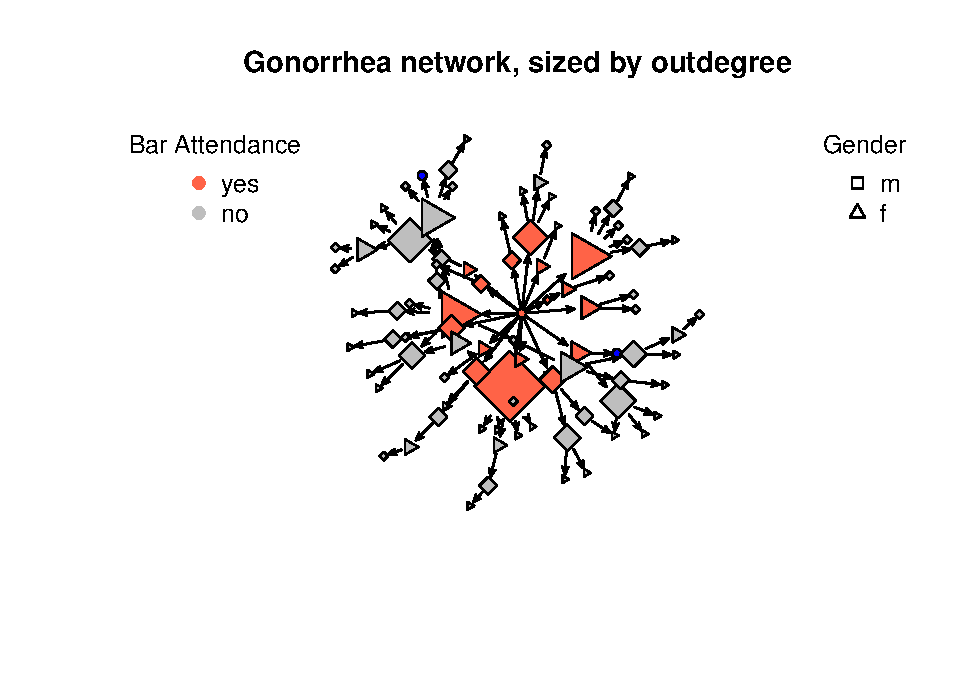
\includegraphics{JStevenRaquel-paper_files/figure-latex/gplot-outdegree-1.pdf}

\hypertarget{principal-component-analysis}{%
\subsection{Principal Component Analysis}\label{principal-component-analysis}}

\begin{Shaded}
\begin{Highlighting}[]
\CommentTok{\# extracting the centralities that were important based on the PCA}
\NormalTok{centrality\_eigen }\OtherTok{\textless{}{-}}\NormalTok{ centralities}\SpecialCharTok{$}\StringTok{\textasciigrave{}}\AttributeTok{eigenvector centralities}\StringTok{\textasciigrave{}}
\NormalTok{centrality\_load }\OtherTok{\textless{}{-}}\NormalTok{ centralities}\SpecialCharTok{$}\StringTok{\textasciigrave{}}\AttributeTok{Load Centrality}\StringTok{\textasciigrave{}}
\NormalTok{centrality\_degree }\OtherTok{\textless{}{-}}\NormalTok{ centralities}\SpecialCharTok{$}\StringTok{\textasciigrave{}}\AttributeTok{Degree Centrality}\StringTok{\textasciigrave{}}
\NormalTok{centrality\_geodesic }\OtherTok{\textless{}{-}}\NormalTok{ centralities}\SpecialCharTok{$}\StringTok{\textasciigrave{}}\AttributeTok{Geodesic K{-}Path Centrality}\StringTok{\textasciigrave{}}
\NormalTok{centrality\_shortest }\OtherTok{\textless{}{-}}\NormalTok{ centralities}\SpecialCharTok{$}\StringTok{\textasciigrave{}}\AttributeTok{Shortest{-}Paths Betweenness Centrality}\StringTok{\textasciigrave{}}
\NormalTok{centrality\_info }\OtherTok{\textless{}{-}}\NormalTok{ centralities}\SpecialCharTok{$}\StringTok{\textasciigrave{}}\AttributeTok{Information Centrality}\StringTok{\textasciigrave{}}
\end{Highlighting}
\end{Shaded}

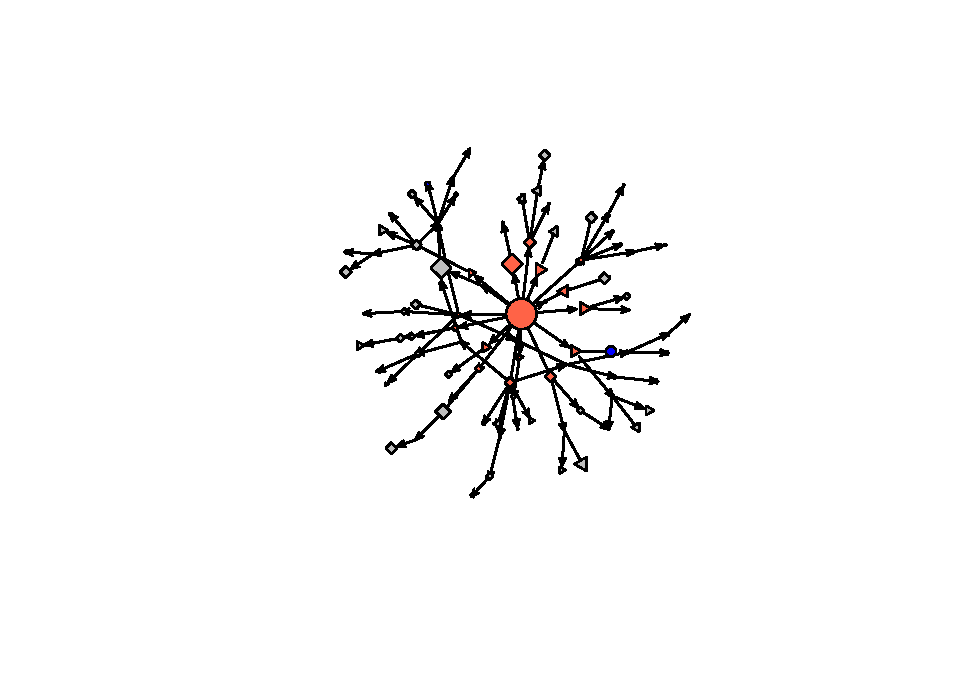
\includegraphics{JStevenRaquel-paper_files/figure-latex/gplot-size-eigenvector-centrality-1.pdf}

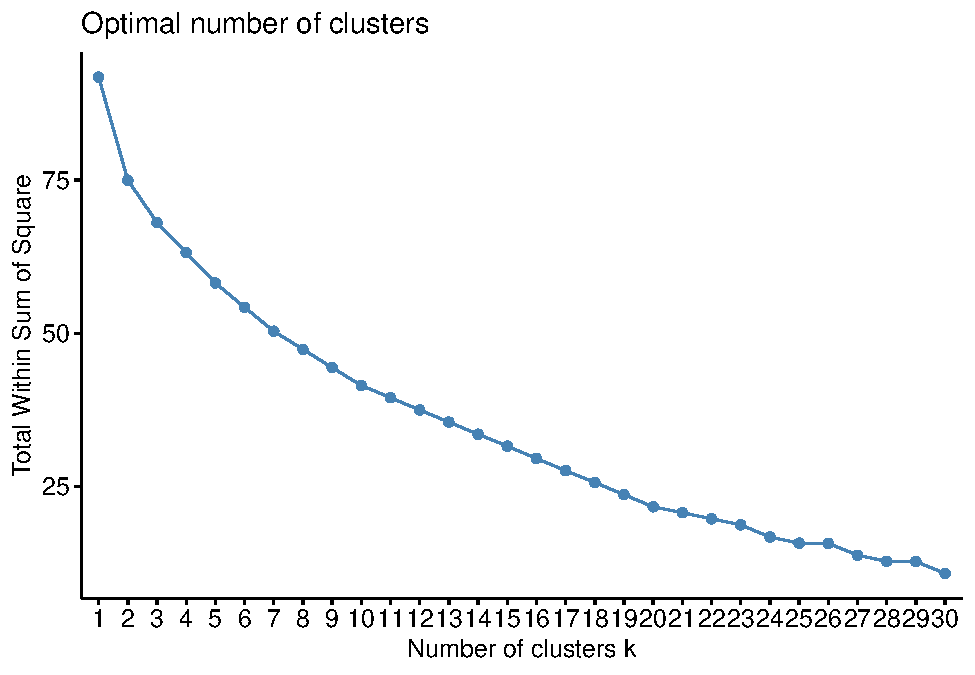
\includegraphics{JStevenRaquel-paper_files/figure-latex/find-best-cluster-number-1.pdf} 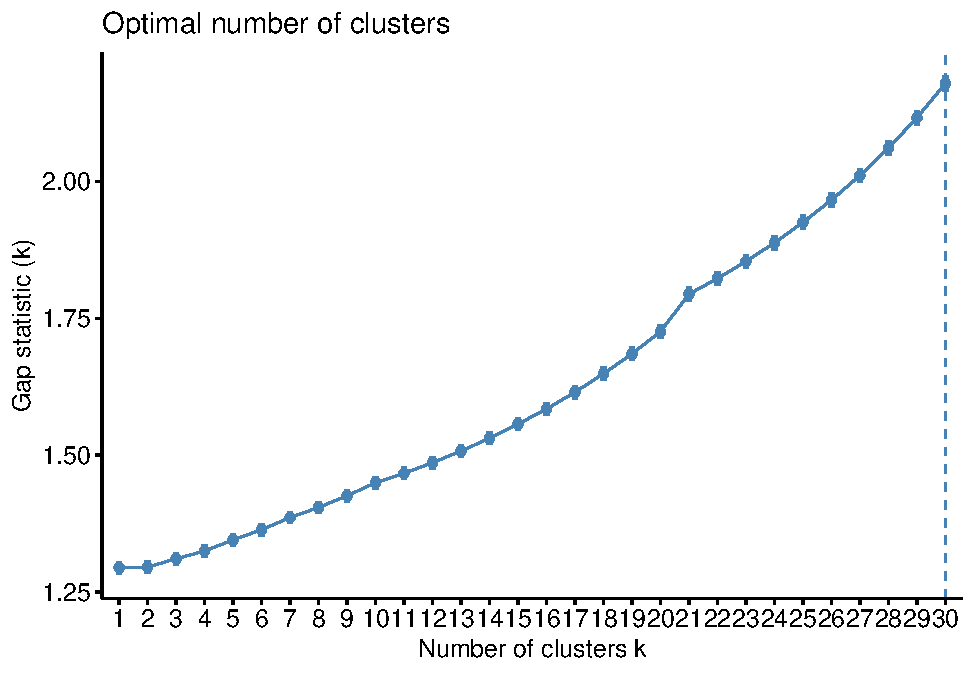
\includegraphics{JStevenRaquel-paper_files/figure-latex/find-best-cluster-number-2.pdf}

\begin{Shaded}
\begin{Highlighting}[]
\NormalTok{km }\OtherTok{\textless{}{-}} \FunctionTok{kmeans}\NormalTok{(gonnet, }\AttributeTok{centers =} \DecValTok{21}\NormalTok{, }\AttributeTok{nstart =} \DecValTok{25}\NormalTok{)}

\CommentTok{\# fviz\_cluster(km, data = gonnet\_nob)}

\CommentTok{\# library(netdiffuseR) is loaded}
\NormalTok{gonnet\_edgelist }\OtherTok{\textless{}{-}} \FunctionTok{adjmat\_to\_edgelist}\NormalTok{(gonnet, }\AttributeTok{undirected =}\NormalTok{ F)}

\CommentTok{\# cluster\_membership}
\NormalTok{km\_cluster\_mem }\OtherTok{\textless{}{-}}\NormalTok{ km}\SpecialCharTok{$}\NormalTok{cluster }\SpecialCharTok{\%\textgreater{}\%} \FunctionTok{as.data.frame}\NormalTok{() }\SpecialCharTok{\%\textgreater{}\%}
\NormalTok{  tibble}\SpecialCharTok{::}\FunctionTok{rownames\_to\_column}\NormalTok{() }\SpecialCharTok{\%\textgreater{}\%}
  \FunctionTok{rename}\NormalTok{(}\AttributeTok{node =} \StringTok{\textquotesingle{}rowname\textquotesingle{}}\NormalTok{, }\AttributeTok{cluster =} \StringTok{\textquotesingle{}.\textquotesingle{}}\NormalTok{)}
\end{Highlighting}
\end{Shaded}

\begin{verbatim}
## [1] 0.8444488
## [1] 0.8528613
## [1] 0.8285892
## [1] 0.8514371
\end{verbatim}

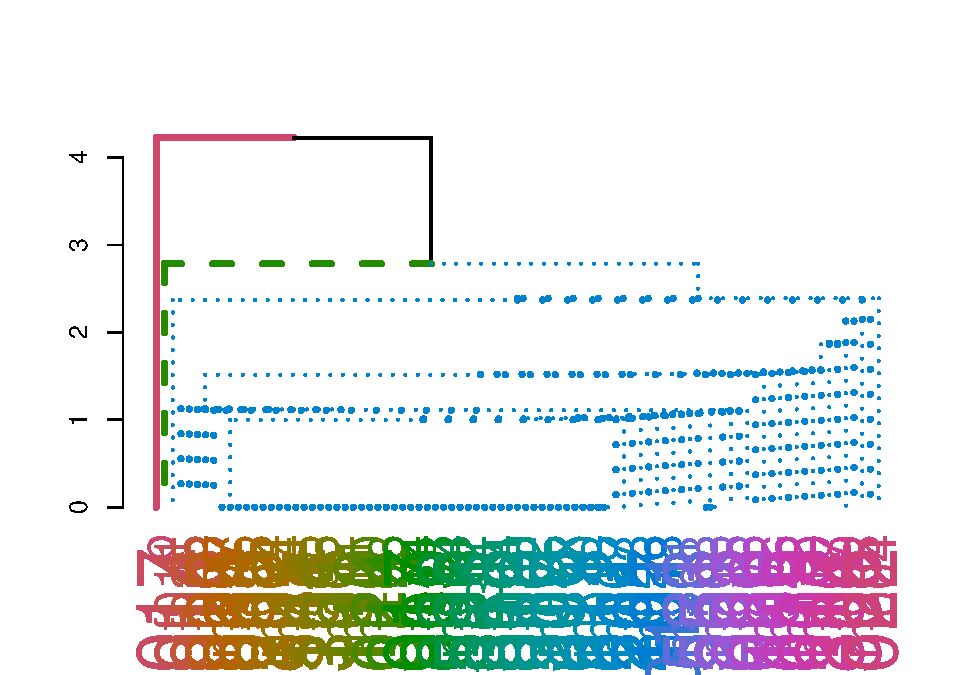
\includegraphics{JStevenRaquel-paper_files/figure-latex/agnes-hclust-1.pdf}

\begin{Shaded}
\begin{Highlighting}[]
\NormalTok{fit }\OtherTok{\textless{}{-}} 
  \FunctionTok{pvclust}\NormalTok{(gonnet, }
  \AttributeTok{method.hclust =} \StringTok{"single"}\NormalTok{,}
  \AttributeTok{method.dist =} \StringTok{"euclidean"}\NormalTok{,}
  \AttributeTok{iseed =} \DecValTok{10}\NormalTok{, }\CommentTok{\# to get same results}
  \AttributeTok{parallel =}\NormalTok{ T, }\CommentTok{\# to use all but one CPU thread}
  \AttributeTok{nboot =} \DecValTok{1000}\NormalTok{) }
\end{Highlighting}
\end{Shaded}

\begin{verbatim}
## Creating a temporary cluster...done:
## socket cluster with 15 nodes on host 'localhost'
## Multiscale bootstrap... Done.
\end{verbatim}

\begin{Shaded}
\begin{Highlighting}[]
\NormalTok{fit\_hclust }\OtherTok{\textless{}{-}}\NormalTok{ fit}\SpecialCharTok{$}\NormalTok{hclust}
\NormalTok{fit\_hclust }\SpecialCharTok{\%\textgreater{}\%} \FunctionTok{cutreeDynamicTree}\NormalTok{(}\AttributeTok{deepSplit =}\NormalTok{ F)}
\end{Highlighting}
\end{Shaded}

\begin{verbatim}
##  [1] 1 1 1 1 1 1 1 1 1 1 1 1 1 1 1 1 1 1 1 1 1 1 1 1 1 1 1 1 1 1 1 1 1 1 1 1 1 1
## [39] 1 1 1 1 1 1 1 1 1 1 1 1 1 1 1 1 1 1 1 1 1 1 1 1 0 1 1 1 1 1 1 1 1 1 1 1 1 1
## [77] 1 1 1 1 1 1 1 1 1 1 1 1 1
\end{verbatim}

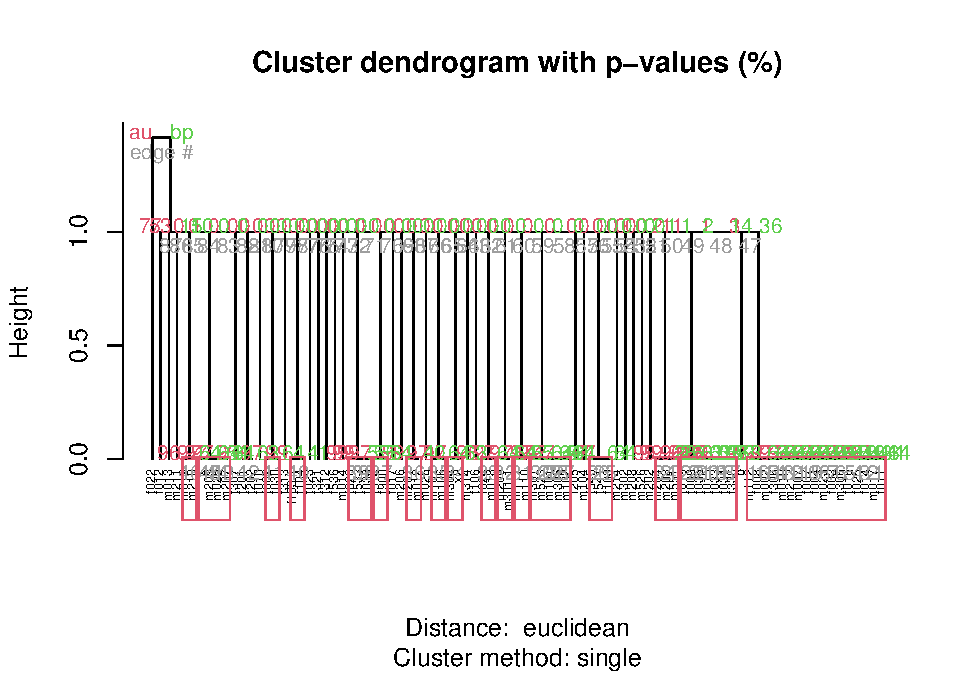
\includegraphics{JStevenRaquel-paper_files/figure-latex/plot-dendrogram-1.pdf}

\begin{verbatim}
## [1] "The mean overall network density is 0.013."
\end{verbatim}

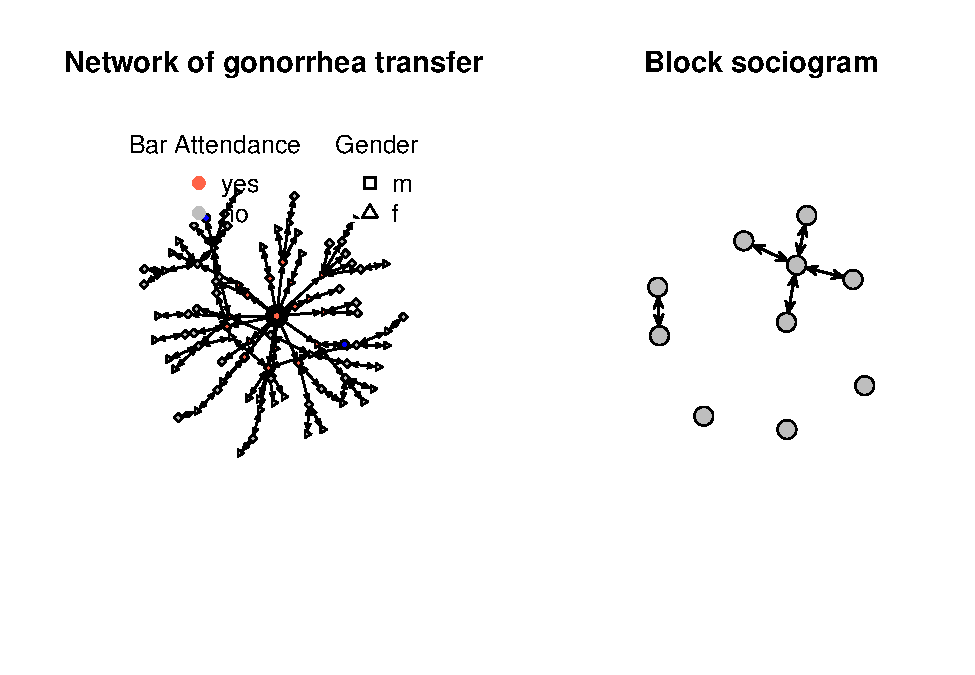
\includegraphics{JStevenRaquel-paper_files/figure-latex/blockmodel-1.pdf}

\begin{verbatim}
## Note: fast-greedy community algorithm is for undirected graphs.
\end{verbatim}

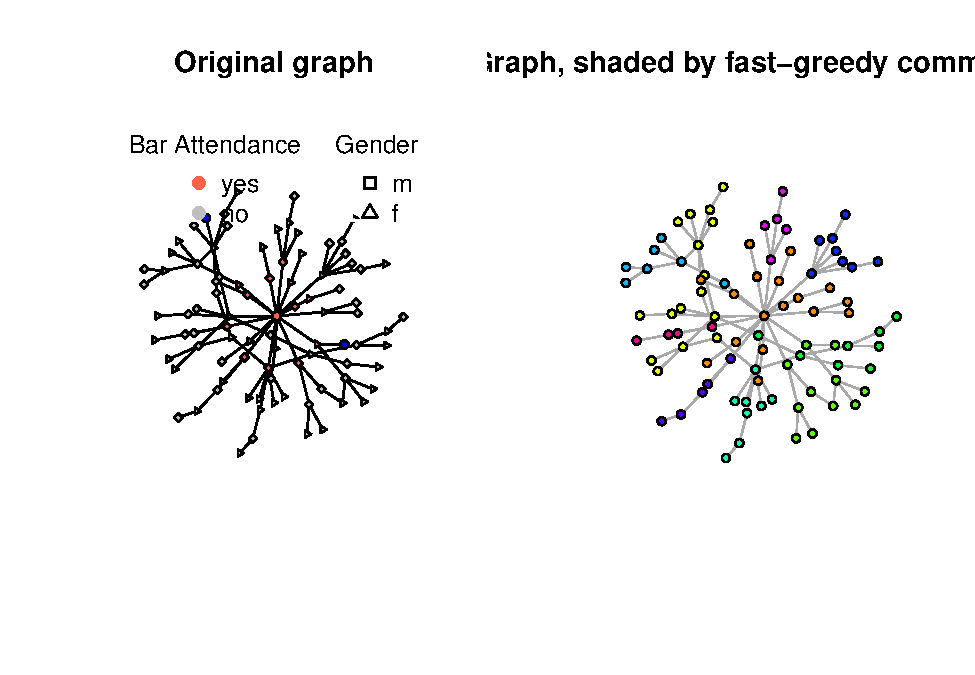
\includegraphics{JStevenRaquel-paper_files/figure-latex/plotting-fast-greedy-community-1.pdf}

\begin{Shaded}
\begin{Highlighting}[]
\FunctionTok{par}\NormalTok{(}\AttributeTok{mfrow =} \FunctionTok{c}\NormalTok{(}\DecValTok{1}\NormalTok{,}\DecValTok{1}\NormalTok{))}
\FunctionTok{set.seed}\NormalTok{(}\DecValTok{10}\NormalTok{)}
\NormalTok{edgelist }\OtherTok{\textless{}{-}} \FunctionTok{as.edgelist}\NormalTok{(gonnet, }\AttributeTok{n =} \FunctionTok{dim}\NormalTok{(gonnet)[}\DecValTok{1}\NormalTok{])}
\FunctionTok{plot\_kcores}\NormalTok{(edgelist, }\AttributeTok{sym =}\NormalTok{ F, }\AttributeTok{mode =} \StringTok{"digraph"}\NormalTok{, }
            \AttributeTok{coord =}\NormalTok{ org\_coord,}
            \AttributeTok{cmode =} \StringTok{"outdegree"}\NormalTok{)}
\end{Highlighting}
\end{Shaded}

\newpage

\hypertarget{references}{%
\section{References}\label{references}}

\newpage

\hypertarget{appendix}{%
\section{Appendix}\label{appendix}}

\begin{Shaded}
\begin{Highlighting}[]
\NormalTok{knitr}\SpecialCharTok{::}\NormalTok{opts\_chunk}\SpecialCharTok{$}\FunctionTok{set}\NormalTok{(}\AttributeTok{echo =} \ConstantTok{TRUE}\NormalTok{)}
\FunctionTok{library}\NormalTok{(tidyverse)}
\FunctionTok{library}\NormalTok{(sna)}
\FunctionTok{library}\NormalTok{(igraph)}
\FunctionTok{library}\NormalTok{(epimdr) }\CommentTok{\# for gonnet data}
\FunctionTok{library}\NormalTok{(pvclust) }\CommentTok{\# for pvclust()}
\FunctionTok{library}\NormalTok{(CINNA) }\CommentTok{\# for pca\_centralities()}
\FunctionTok{library}\NormalTok{(car) }\CommentTok{\# for leveneTest()}
\FunctionTok{library}\NormalTok{(factoextra) }\CommentTok{\# for nbclust}
\FunctionTok{library}\NormalTok{(cluster) }\CommentTok{\# more cluster analysis}
\FunctionTok{library}\NormalTok{(netdiffuseR)}
\FunctionTok{library}\NormalTok{(dendextend) }\CommentTok{\# for appealing dendrograms}
\FunctionTok{library}\NormalTok{(dynamicTreeCut)}
\FunctionTok{data}\NormalTok{(gonnet)}
\FunctionTok{source}\NormalTok{(here}\SpecialCharTok{::}\FunctionTok{here}\NormalTok{(}\StringTok{"functions.R"}\NormalTok{))}
\CommentTok{\# data is loaded as \textquotesingle{}gonnet\textquotesingle{}}
\NormalTok{nodes }\OtherTok{\textless{}{-}} \FunctionTok{rownames}\NormalTok{(gonnet)}
\FunctionTok{colnames}\NormalTok{(gonnet) }\OtherTok{\textless{}{-}}\NormalTok{ nodes}

\CommentTok{\# symmetrized graph (undirected)}
\NormalTok{gonnet\_sym }\OtherTok{\textless{}{-}} \FunctionTok{symmetrize}\NormalTok{(gonnet, }\AttributeTok{rule =} \StringTok{"weak"}\NormalTok{)}

\NormalTok{gonnet\_df }\OtherTok{\textless{}{-}} \FunctionTok{data.frame}\NormalTok{(nodes) }\SpecialCharTok{\%\textgreater{}\%}
  \FunctionTok{mutate}\NormalTok{(}\AttributeTok{gender =} \FunctionTok{ifelse}\NormalTok{(}\FunctionTok{grepl}\NormalTok{(}\StringTok{"m"}\NormalTok{, nodes), }\AttributeTok{yes =} \StringTok{"m"}\NormalTok{, }\AttributeTok{no =} \ConstantTok{NA}\NormalTok{)) }\SpecialCharTok{\%\textgreater{}\%}
  \FunctionTok{mutate}\NormalTok{(}\AttributeTok{gender =} \FunctionTok{ifelse}\NormalTok{(}\FunctionTok{grepl}\NormalTok{(}\StringTok{"f"}\NormalTok{, nodes), }\AttributeTok{yes =} \StringTok{"f"}\NormalTok{, }\AttributeTok{no =}\NormalTok{ gender)) }\SpecialCharTok{\%\textgreater{}\%}
  \FunctionTok{mutate}\NormalTok{(}\AttributeTok{gender\_lty =} \FunctionTok{ifelse}\NormalTok{(gender }\SpecialCharTok{==} \StringTok{"m"}\NormalTok{, }\AttributeTok{yes =} \DecValTok{4}\NormalTok{, }\AttributeTok{no =} \DecValTok{3}\NormalTok{)) }\SpecialCharTok{\%\textgreater{}\%}
  \FunctionTok{mutate}\NormalTok{(}\AttributeTok{gender\_lty =} \FunctionTok{ifelse}\NormalTok{(gender }\SpecialCharTok{==} \StringTok{"f"}\NormalTok{, }\AttributeTok{yes =} \DecValTok{3}\NormalTok{, }\AttributeTok{no =}\NormalTok{ gender\_lty)) }\SpecialCharTok{\%\textgreater{}\%}
  \FunctionTok{mutate}\NormalTok{(}\AttributeTok{gender\_lty =} \FunctionTok{ifelse}\NormalTok{(gender }\SpecialCharTok{\%in\%} \FunctionTok{c}\NormalTok{(}\StringTok{"m"}\NormalTok{, }\StringTok{"f"}\NormalTok{), }\AttributeTok{yes =}\NormalTok{ gender\_lty, }\AttributeTok{no =} \DecValTok{50}\NormalTok{)}
\NormalTok{         ) }\SpecialCharTok{\%\textgreater{}\%}
  \FunctionTok{mutate}\NormalTok{(}\AttributeTok{attended\_bar =}\NormalTok{ gonnet[}\StringTok{"b"}\NormalTok{,] }\SpecialCharTok{==} \DecValTok{1}\NormalTok{) }\SpecialCharTok{\%\textgreater{}\%}
  \FunctionTok{mutate}\NormalTok{(}\AttributeTok{col =} \FunctionTok{ifelse}\NormalTok{(attended\_bar }\SpecialCharTok{==}\NormalTok{ T, }\StringTok{"tomato1"}\NormalTok{, }\StringTok{"grey"}\NormalTok{))}


\NormalTok{gonnet\_df}\SpecialCharTok{$}\NormalTok{col[}\SpecialCharTok{!}\NormalTok{(gonnet\_df}\SpecialCharTok{$}\NormalTok{gender }\SpecialCharTok{\%in\%} \FunctionTok{c}\NormalTok{(}\StringTok{"m"}\NormalTok{, }\StringTok{"f"}\NormalTok{))] }\OtherTok{\textless{}{-}} \StringTok{"blue"}
\NormalTok{gonnet\_df}\SpecialCharTok{$}\NormalTok{col[gonnet\_df}\SpecialCharTok{$}\NormalTok{nodes }\SpecialCharTok{==} \StringTok{"b"}\NormalTok{] }\OtherTok{\textless{}{-}} \StringTok{"tomato1"}
\FunctionTok{par}\NormalTok{(}\AttributeTok{mfrow =} \FunctionTok{c}\NormalTok{(}\DecValTok{1}\NormalTok{,}\DecValTok{1}\NormalTok{))}
\FunctionTok{set.seed}\NormalTok{(}\DecValTok{10}\NormalTok{)}
\NormalTok{org\_coord }\OtherTok{\textless{}{-}} 
  \FunctionTok{gplot}\NormalTok{(gonnet, }\AttributeTok{vertex.col =}\NormalTok{ gonnet\_df}\SpecialCharTok{$}\NormalTok{col,}
      \AttributeTok{vertex.sides =}\NormalTok{ gonnet\_df}\SpecialCharTok{$}\NormalTok{gender\_lty,}
      \AttributeTok{displaylabels =}\NormalTok{ T, }\AttributeTok{label.cex =} \FloatTok{0.6}\NormalTok{,}
      \AttributeTok{boxed.labels =}\NormalTok{ F, }\AttributeTok{pad =} \DecValTok{2}\NormalTok{, }\AttributeTok{usearrows =}\NormalTok{ T,}
      \AttributeTok{vertex.cex =} \FloatTok{1.25}\NormalTok{)}
\CommentTok{\# legend for gender}
\FunctionTok{legend}\NormalTok{(}\StringTok{"topleft"}\NormalTok{,}
       \AttributeTok{legend =} \FunctionTok{c}\NormalTok{(}\StringTok{"yes"}\NormalTok{, }\StringTok{"no"}\NormalTok{),}
       \AttributeTok{col =} \FunctionTok{c}\NormalTok{(}\StringTok{"tomato1"}\NormalTok{, }\StringTok{"grey"}\NormalTok{),}
       \AttributeTok{fill =}\NormalTok{ F, }\AttributeTok{border =} \StringTok{"white"}\NormalTok{, }\AttributeTok{pch =} \DecValTok{19}\NormalTok{,}
       \AttributeTok{title =} \StringTok{"Bar Attendance"}\NormalTok{, }\AttributeTok{bty =} \StringTok{"n"}\NormalTok{)}
\FunctionTok{legend}\NormalTok{(}\StringTok{"topright"}\NormalTok{,}
       \AttributeTok{legend =} \FunctionTok{c}\NormalTok{(}\StringTok{"m"}\NormalTok{, }\StringTok{"f"}\NormalTok{),}
       \AttributeTok{col =} \FunctionTok{c}\NormalTok{(}\StringTok{"black"}\NormalTok{),}
       \AttributeTok{fill =}\NormalTok{ F, }\AttributeTok{border =} \StringTok{"white"}\NormalTok{, }\AttributeTok{pch =} \FunctionTok{c}\NormalTok{(}\DecValTok{0}\NormalTok{, }\DecValTok{2}\NormalTok{),}
       \AttributeTok{title =} \StringTok{"Gender"}\NormalTok{, }\AttributeTok{bty =} \StringTok{"n"}\NormalTok{)}
\CommentTok{\# legend for bar attendance}
\NormalTok{cen }\OtherTok{\textless{}{-}} \FunctionTok{get\_centralities}\NormalTok{(gonnet, }\StringTok{"directed"}\NormalTok{)}

\CommentTok{\# correlations between centrality measures}
\FunctionTok{centrality\_correlations}\NormalTok{(gonnet, cen)}

\NormalTok{cen\_sym }\OtherTok{\textless{}{-}} \FunctionTok{get\_centralities}\NormalTok{(gonnet\_sym, }\StringTok{"undirected"}\NormalTok{)}
\FunctionTok{centrality\_correlations}\NormalTok{(gonnet\_sym, cen\_sym)}
\CommentTok{\# creating igraph object}
\NormalTok{gonnet\_ig }\OtherTok{\textless{}{-}} \FunctionTok{graph\_from\_adjacency\_matrix}\NormalTok{(gonnet)}

\NormalTok{(pc }\OtherTok{\textless{}{-}} \FunctionTok{proper\_centralities}\NormalTok{(gonnet\_ig)) }\SpecialCharTok{\%\textgreater{}\%} 
  \FunctionTok{capture.output}\NormalTok{() }\SpecialCharTok{\%\textgreater{}\%}
  \FunctionTok{invisible}\NormalTok{()}

\NormalTok{centralities }\OtherTok{\textless{}{-}} \FunctionTok{calculate\_centralities}\NormalTok{(gonnet\_ig, }
                       \AttributeTok{include =}\NormalTok{ pc[}\FunctionTok{c}\NormalTok{(}\DecValTok{1}\NormalTok{, }\DecValTok{4}\NormalTok{, }\DecValTok{11}\NormalTok{, }\DecValTok{16}\NormalTok{, }\DecValTok{27}\NormalTok{, }
                                      \DecValTok{45}\NormalTok{, }\DecValTok{8}\NormalTok{, }\DecValTok{18}\NormalTok{, }\DecValTok{31}\NormalTok{, }\DecValTok{43}\NormalTok{, }\DecValTok{3}\NormalTok{, }\DecValTok{19}\NormalTok{)])}

\CommentTok{\# plot of different centralities\textquotesingle{} contributions via PCA}
\FunctionTok{pca\_centralities}\NormalTok{(centralities)}

\NormalTok{gonnet\_df2 }\OtherTok{\textless{}{-}} \FunctionTok{cbind}\NormalTok{(gonnet\_df, cen) }\SpecialCharTok{\%\textgreater{}\%} \FunctionTok{select}\NormalTok{(}\SpecialCharTok{{-}}\NormalTok{id)}

\CommentTok{\# boxplot comparing outdegree}
\NormalTok{outdegree\_gender }\OtherTok{\textless{}{-}}\NormalTok{ gonnet\_df2 }\SpecialCharTok{\%\textgreater{}\%} 
  \FunctionTok{select}\NormalTok{(nodes, gender, outdegree) }\SpecialCharTok{\%\textgreater{}\%} 
  \FunctionTok{drop\_na}\NormalTok{()}

\CommentTok{\# boxplot of outdegree by gender}
\FunctionTok{ggplot}\NormalTok{(outdegree\_gender, }\FunctionTok{aes}\NormalTok{(}\AttributeTok{x=}\NormalTok{gender, }\AttributeTok{y=}\NormalTok{outdegree)) }\SpecialCharTok{+} 
  \FunctionTok{geom\_boxplot}\NormalTok{()}

\CommentTok{\# average outdegree overall}
\NormalTok{gonnet\_df2}\SpecialCharTok{$}\NormalTok{outdegree }\SpecialCharTok{\%\textgreater{}\%} \FunctionTok{mean}\NormalTok{()}

\CommentTok{\# average outdegree among males in network, overall}
\NormalTok{outdegree\_m }\OtherTok{\textless{}{-}}\NormalTok{ gonnet\_df2 }\SpecialCharTok{\%\textgreater{}\%}
  \FunctionTok{select}\NormalTok{(nodes, gender, outdegree) }\SpecialCharTok{\%\textgreater{}\%}
  \FunctionTok{filter}\NormalTok{(gender }\SpecialCharTok{==} \StringTok{"m"}\NormalTok{) }\SpecialCharTok{\%\textgreater{}\%}
  \FunctionTok{select}\NormalTok{(outdegree) }\SpecialCharTok{\%\textgreater{}\%} 
  \FunctionTok{unlist}\NormalTok{()}
\NormalTok{outdegree\_m }\SpecialCharTok{\%\textgreater{}\%} \FunctionTok{mean}\NormalTok{()}
\NormalTok{outdegree\_m }\SpecialCharTok{\%\textgreater{}\%} \FunctionTok{median}\NormalTok{()}
\CommentTok{\# male outdegree that excludes nodes with zero outdegree}
\NormalTok{gonnet\_df2 }\SpecialCharTok{\%\textgreater{}\%}
  \FunctionTok{select}\NormalTok{(nodes, gender, outdegree) }\SpecialCharTok{\%\textgreater{}\%}
  \FunctionTok{filter}\NormalTok{(gender }\SpecialCharTok{==} \StringTok{"m"} \SpecialCharTok{\&}\NormalTok{ outdegree }\SpecialCharTok{!=} \DecValTok{0}\NormalTok{) }\SpecialCharTok{\%\textgreater{}\%}
  \FunctionTok{select}\NormalTok{(outdegree) }\SpecialCharTok{\%\textgreater{}\%}
  \FunctionTok{unlist}\NormalTok{() }\SpecialCharTok{\%\textgreater{}\%} \FunctionTok{mean}\NormalTok{()}

\CommentTok{\# average outdegree among females}
\NormalTok{outdegree\_f }\OtherTok{\textless{}{-}}\NormalTok{ gonnet\_df2 }\SpecialCharTok{\%\textgreater{}\%} 
  \FunctionTok{select}\NormalTok{(nodes, gender, outdegree) }\SpecialCharTok{\%\textgreater{}\%}
  \FunctionTok{filter}\NormalTok{(gender }\SpecialCharTok{==} \StringTok{"f"}\NormalTok{) }\SpecialCharTok{\%\textgreater{}\%} 
  \FunctionTok{select}\NormalTok{(outdegree) }\SpecialCharTok{\%\textgreater{}\%}
  \FunctionTok{unlist}\NormalTok{()}
\NormalTok{outdegree\_f }\SpecialCharTok{\%\textgreater{}\%} \FunctionTok{mean}\NormalTok{()}
\NormalTok{outdegree\_f }\SpecialCharTok{\%\textgreater{}\%} \FunctionTok{median}\NormalTok{()}

\CommentTok{\# female outdegree that excludes nodes with zero outdegree}
\NormalTok{gonnet\_df2 }\SpecialCharTok{\%\textgreater{}\%}
  \FunctionTok{select}\NormalTok{(nodes, gender, outdegree) }\SpecialCharTok{\%\textgreater{}\%}
  \FunctionTok{filter}\NormalTok{(gender }\SpecialCharTok{==} \StringTok{"f"} \SpecialCharTok{\&}\NormalTok{ outdegree }\SpecialCharTok{!=} \DecValTok{0}\NormalTok{) }\SpecialCharTok{\%\textgreater{}\%}
  \FunctionTok{select}\NormalTok{(outdegree) }\SpecialCharTok{\%\textgreater{}\%}
  \FunctionTok{unlist}\NormalTok{() }\SpecialCharTok{\%\textgreater{}\%} \FunctionTok{mean}\NormalTok{()}
\CommentTok{\# levene test for equality of variances}
\CommentTok{\# H0: the variance in outdegree between the two genders is equal}
\NormalTok{outdegree\_gender}\SpecialCharTok{$}\NormalTok{gender }\OtherTok{\textless{}{-}} \FunctionTok{as.factor}\NormalTok{(outdegree\_gender}\SpecialCharTok{$}\NormalTok{gender)}
  
\FunctionTok{leveneTest}\NormalTok{(outdegree }\SpecialCharTok{\textasciitilde{}}\NormalTok{ gender, }
           \AttributeTok{data =}\NormalTok{ outdegree\_gender)}
\CommentTok{\# p{-}value \textgreater{} 0.05, so we fail to reject H0, conclude the variances are equal}
\CommentTok{\# Student\textquotesingle{}s t{-}test comparing the mean outdegree of men and women}
\CommentTok{\# H0: mu\_x {-} mu\_y = 0}
\FunctionTok{t.test}\NormalTok{(}\AttributeTok{x =}\NormalTok{ outdegree\_m, }
       \AttributeTok{y =}\NormalTok{ outdegree\_f,}
       \AttributeTok{var.equal =}\NormalTok{ T, }\AttributeTok{alternative =} \StringTok{"two.sided"}\NormalTok{)}
\CommentTok{\# p{-}value = 0.5232 \textgreater{} 0.05, we fail to reject H0}


\CommentTok{\# boxplot comparing distribution of outdegree between bar (not){-}attended}
\FunctionTok{ggplot}\NormalTok{(gonnet\_df2 }\SpecialCharTok{\%\textgreater{}\%} \FunctionTok{filter}\NormalTok{(}\SpecialCharTok{!}\NormalTok{(nodes }\SpecialCharTok{\%in\%} \FunctionTok{c}\NormalTok{(}\StringTok{"b"}\NormalTok{, }\StringTok{"x"}\NormalTok{, }\StringTok{"x2"}\NormalTok{))), }
       \FunctionTok{aes}\NormalTok{(}\AttributeTok{x =}\NormalTok{ attended\_bar, outdegree)) }\SpecialCharTok{+} 
  \FunctionTok{geom\_boxplot}\NormalTok{() }\SpecialCharTok{+} \FunctionTok{theme\_bw}\NormalTok{()}

\CommentTok{\# average outdegree among bar attendees}
\NormalTok{outdegree\_bar }\OtherTok{\textless{}{-}}\NormalTok{ gonnet\_df2 }\SpecialCharTok{\%\textgreater{}\%} 
  \FunctionTok{select}\NormalTok{(nodes, attended\_bar, outdegree) }\SpecialCharTok{\%\textgreater{}\%}
  \FunctionTok{filter}\NormalTok{(}\SpecialCharTok{!}\NormalTok{(nodes }\SpecialCharTok{\%in\%} \FunctionTok{c}\NormalTok{(}\StringTok{"b"}\NormalTok{, }\StringTok{"x2"}\NormalTok{, }\StringTok{"x"}\NormalTok{))) }\SpecialCharTok{\%\textgreater{}\%}
  \FunctionTok{filter}\NormalTok{(attended\_bar }\SpecialCharTok{==} \ConstantTok{TRUE}\NormalTok{)}

\CommentTok{\# average outdegree among non{-}bar attendees}
\NormalTok{outdegree\_nobar }\OtherTok{\textless{}{-}}\NormalTok{ gonnet\_df2 }\SpecialCharTok{\%\textgreater{}\%} 
  \FunctionTok{select}\NormalTok{(nodes, attended\_bar, outdegree) }\SpecialCharTok{\%\textgreater{}\%}
  \FunctionTok{filter}\NormalTok{(}\SpecialCharTok{!}\NormalTok{(nodes }\SpecialCharTok{\%in\%} \FunctionTok{c}\NormalTok{(}\StringTok{"b"}\NormalTok{, }\StringTok{"x2"}\NormalTok{, }\StringTok{"x"}\NormalTok{))) }\SpecialCharTok{\%\textgreater{}\%}
  \FunctionTok{filter}\NormalTok{(attended\_bar }\SpecialCharTok{==} \ConstantTok{FALSE}\NormalTok{)}

\CommentTok{\# sample sizes are unequal, so we cannot assume equal variance}
\CommentTok{\# try two{-}sided Welch\textquotesingle{}s t.test}
\CommentTok{\# H0: mu\_x {-} mu\_y = 0}
\FunctionTok{t.test}\NormalTok{(}\AttributeTok{x =}\NormalTok{ outdegree\_bar}\SpecialCharTok{$}\NormalTok{outdegree,}
       \AttributeTok{y =}\NormalTok{ outdegree\_nobar}\SpecialCharTok{$}\NormalTok{outdegree,}
       \AttributeTok{var.equal =} \ConstantTok{FALSE}\NormalTok{, }\AttributeTok{alternative =} \StringTok{"two.sided"}\NormalTok{)}
\CommentTok{\# p{-}value \textless{} 0.05, reject H0}
\CommentTok{\# conclude the difference in mean outdegree is not equal to zero}
\CommentTok{\# normalizing the outdegree of bar because of course it has a high outdegree}
\NormalTok{outdegree\_m }\OtherTok{\textless{}{-}}\NormalTok{ cen}\SpecialCharTok{$}\NormalTok{outdegree }\SpecialCharTok{+} \DecValTok{1}
\NormalTok{outdegree\_m[}\DecValTok{1}\NormalTok{] }\OtherTok{\textless{}{-}} \DecValTok{1}

\FunctionTok{set.seed}\NormalTok{(}\DecValTok{10}\NormalTok{)}

\CommentTok{\# plotting based on outdegree}
\FunctionTok{gplot}\NormalTok{(gonnet, }
      \AttributeTok{vertex.col =}\NormalTok{ gonnet\_df}\SpecialCharTok{$}\NormalTok{col,}
      \AttributeTok{vertex.sides =}\NormalTok{ gonnet\_df}\SpecialCharTok{$}\NormalTok{gender\_lty,}
      \AttributeTok{vertex.cex =}\NormalTok{ outdegree\_m,}
      \AttributeTok{coord =}\NormalTok{ org\_coord)}
\CommentTok{\# legend for gender}
\FunctionTok{legend}\NormalTok{(}\StringTok{"topleft"}\NormalTok{,}
       \AttributeTok{legend =} \FunctionTok{c}\NormalTok{(}\StringTok{"yes"}\NormalTok{, }\StringTok{"no"}\NormalTok{),}
       \AttributeTok{col =} \FunctionTok{c}\NormalTok{(}\StringTok{"tomato1"}\NormalTok{, }\StringTok{"grey"}\NormalTok{),}
       \AttributeTok{fill =}\NormalTok{ F, }\AttributeTok{border =} \StringTok{"white"}\NormalTok{, }\AttributeTok{pch =} \DecValTok{19}\NormalTok{,}
       \AttributeTok{title =} \StringTok{"Bar Attendance"}\NormalTok{, }\AttributeTok{bty =} \StringTok{"n"}\NormalTok{)}
\FunctionTok{legend}\NormalTok{(}\StringTok{"topright"}\NormalTok{,}
       \AttributeTok{legend =} \FunctionTok{c}\NormalTok{(}\StringTok{"m"}\NormalTok{, }\StringTok{"f"}\NormalTok{),}
       \AttributeTok{col =} \FunctionTok{c}\NormalTok{(}\StringTok{"black"}\NormalTok{),}
       \AttributeTok{fill =}\NormalTok{ F, }\AttributeTok{border =} \StringTok{"white"}\NormalTok{, }\AttributeTok{pch =} \FunctionTok{c}\NormalTok{(}\DecValTok{0}\NormalTok{, }\DecValTok{2}\NormalTok{),}
       \AttributeTok{title =} \StringTok{"Gender"}\NormalTok{, }\AttributeTok{bty =} \StringTok{"n"}\NormalTok{)}
\FunctionTok{title}\NormalTok{(}\StringTok{"Gonorrhea network, sized by outdegree"}\NormalTok{)}
\CommentTok{\# extracting the centralities that were important based on the PCA}
\NormalTok{centrality\_eigen }\OtherTok{\textless{}{-}}\NormalTok{ centralities}\SpecialCharTok{$}\StringTok{\textasciigrave{}}\AttributeTok{eigenvector centralities}\StringTok{\textasciigrave{}}
\NormalTok{centrality\_load }\OtherTok{\textless{}{-}}\NormalTok{ centralities}\SpecialCharTok{$}\StringTok{\textasciigrave{}}\AttributeTok{Load Centrality}\StringTok{\textasciigrave{}}
\NormalTok{centrality\_degree }\OtherTok{\textless{}{-}}\NormalTok{ centralities}\SpecialCharTok{$}\StringTok{\textasciigrave{}}\AttributeTok{Degree Centrality}\StringTok{\textasciigrave{}}
\NormalTok{centrality\_geodesic }\OtherTok{\textless{}{-}}\NormalTok{ centralities}\SpecialCharTok{$}\StringTok{\textasciigrave{}}\AttributeTok{Geodesic K{-}Path Centrality}\StringTok{\textasciigrave{}}
\NormalTok{centrality\_shortest }\OtherTok{\textless{}{-}}\NormalTok{ centralities}\SpecialCharTok{$}\StringTok{\textasciigrave{}}\AttributeTok{Shortest{-}Paths Betweenness Centrality}\StringTok{\textasciigrave{}}
\NormalTok{centrality\_info }\OtherTok{\textless{}{-}}\NormalTok{ centralities}\SpecialCharTok{$}\StringTok{\textasciigrave{}}\AttributeTok{Information Centrality}\StringTok{\textasciigrave{}}
\FunctionTok{set.seed}\NormalTok{(}\DecValTok{10}\NormalTok{)}

\NormalTok{centrality\_degree[}\DecValTok{1}\NormalTok{] }\OtherTok{\textless{}{-}} \DecValTok{1}
\FunctionTok{gplot}\NormalTok{(gonnet, }\AttributeTok{vertex.col =}\NormalTok{ gonnet\_df}\SpecialCharTok{$}\NormalTok{col,}
      \AttributeTok{vertex.sides =}\NormalTok{ gonnet\_df}\SpecialCharTok{$}\NormalTok{gender\_lty,}
      \AttributeTok{vertex.cex =}\NormalTok{ centrality\_info }\SpecialCharTok{\%\textgreater{}\%} \FunctionTok{scale}\NormalTok{(),}
      \CommentTok{\# displaylabels = T, label.cex = 0.6, label.pos = 2,}
      \AttributeTok{boxed.labels =}\NormalTok{ F, }\AttributeTok{pad =} \DecValTok{2}\NormalTok{,}
      \AttributeTok{coord =}\NormalTok{ org\_coord)}
\CommentTok{\# library(factoextra) is loaded}
\FunctionTok{fviz\_nbclust}\NormalTok{(gonnet, kmeans, }\AttributeTok{method =} \StringTok{"wss"}\NormalTok{, }\AttributeTok{k.max =} \DecValTok{30}\NormalTok{)}

\CommentTok{\# library(cluster) is loaded}
\NormalTok{gap\_stat }\OtherTok{\textless{}{-}} \FunctionTok{clusGap}\NormalTok{(gonnet, }\AttributeTok{FUN =}\NormalTok{ kmeans, }\AttributeTok{nstart =} \DecValTok{25}\NormalTok{, }\AttributeTok{K.max =} \DecValTok{30}\NormalTok{, }\AttributeTok{B =} \DecValTok{50}\NormalTok{)}
\FunctionTok{fviz\_gap\_stat}\NormalTok{(gap\_stat)}
\NormalTok{km }\OtherTok{\textless{}{-}} \FunctionTok{kmeans}\NormalTok{(gonnet, }\AttributeTok{centers =} \DecValTok{21}\NormalTok{, }\AttributeTok{nstart =} \DecValTok{25}\NormalTok{)}

\CommentTok{\# fviz\_cluster(km, data = gonnet\_nob)}

\CommentTok{\# library(netdiffuseR) is loaded}
\NormalTok{gonnet\_edgelist }\OtherTok{\textless{}{-}} \FunctionTok{adjmat\_to\_edgelist}\NormalTok{(gonnet, }\AttributeTok{undirected =}\NormalTok{ F)}

\CommentTok{\# cluster\_membership}
\NormalTok{km\_cluster\_mem }\OtherTok{\textless{}{-}}\NormalTok{ km}\SpecialCharTok{$}\NormalTok{cluster }\SpecialCharTok{\%\textgreater{}\%} \FunctionTok{as.data.frame}\NormalTok{() }\SpecialCharTok{\%\textgreater{}\%}
\NormalTok{  tibble}\SpecialCharTok{::}\FunctionTok{rownames\_to\_column}\NormalTok{() }\SpecialCharTok{\%\textgreater{}\%}
  \FunctionTok{rename}\NormalTok{(}\AttributeTok{node =} \StringTok{\textquotesingle{}rowname\textquotesingle{}}\NormalTok{, }\AttributeTok{cluster =} \StringTok{\textquotesingle{}.\textquotesingle{}}\NormalTok{)}

\FunctionTok{set.seed}\NormalTok{(}\DecValTok{10}\NormalTok{)}
\FunctionTok{par}\NormalTok{(}\AttributeTok{mfrow =} \FunctionTok{c}\NormalTok{(}\DecValTok{1}\NormalTok{,}\DecValTok{1}\NormalTok{))}
\NormalTok{clust }\OtherTok{\textless{}{-}} \FunctionTok{hclust}\NormalTok{(}\FunctionTok{dist}\NormalTok{(gonnet), }\AttributeTok{method =} \StringTok{"average"}\NormalTok{)}
\NormalTok{clust\_dend }\OtherTok{\textless{}{-}}\NormalTok{ clust }\SpecialCharTok{\%\textgreater{}\%} \FunctionTok{as.dendrogram}\NormalTok{()}
\CommentTok{\# clust \textless{}{-} equiv.clust(gonnet)}

\NormalTok{bm\_complete }\OtherTok{\textless{}{-}} \FunctionTok{blockmodel}\NormalTok{(gonnet,}
                          \AttributeTok{ec =}\NormalTok{ clust, }\AttributeTok{k =} \DecValTok{15}\NormalTok{)}

\NormalTok{bmR\_complete }\OtherTok{\textless{}{-}} \FunctionTok{reorder\_blockmodel}\NormalTok{(bm\_complete)}
\CommentTok{\# overall network density, which we will use for alpha}
\NormalTok{alpha }\OtherTok{\textless{}{-}}\NormalTok{ bmR\_complete}\SpecialCharTok{$}\NormalTok{block.model }\SpecialCharTok{\%\textgreater{}\%} \FunctionTok{mean}\NormalTok{(}\AttributeTok{na.rm =}\NormalTok{ T)}
\FunctionTok{paste0}\NormalTok{(}\StringTok{"The mean overall network density is "}\NormalTok{, }\FunctionTok{round}\NormalTok{(alpha, }\DecValTok{3}\NormalTok{), }\StringTok{"."}\NormalTok{)}

\NormalTok{density\_matrix }\OtherTok{\textless{}{-}}\NormalTok{ bmR\_complete}\SpecialCharTok{$}\NormalTok{block.model}
\CommentTok{\# plotting blockmodel }
\FunctionTok{gplot}\NormalTok{(density\_matrix }\SpecialCharTok{\textgreater{}}\NormalTok{ alpha,}
      \AttributeTok{diag =}\NormalTok{ T,}
      \AttributeTok{vertex.cex =} \FloatTok{1.5}\NormalTok{,}
      \AttributeTok{label =} \FunctionTok{unique}\NormalTok{(bmR\_complete}\SpecialCharTok{$}\NormalTok{block.membership),}
      \CommentTok{\# boxed.labels=F,}
      \AttributeTok{vertex.col=}\StringTok{"grey"}\NormalTok{,}
      \AttributeTok{pad =} \FloatTok{1.25}\NormalTok{)}
\FunctionTok{title}\NormalTok{(}\StringTok{"Block sociogram"}\NormalTok{)}
\FunctionTok{set.seed}\NormalTok{(}\DecValTok{10}\NormalTok{)}
\FunctionTok{par}\NormalTok{(}\AttributeTok{mfrow =} \FunctionTok{c}\NormalTok{(}\DecValTok{1}\NormalTok{,}\DecValTok{1}\NormalTok{))}
\CommentTok{\#define linkage methods}
\NormalTok{hclust\_methods }\OtherTok{\textless{}{-}} \FunctionTok{c}\NormalTok{(}\StringTok{"average"}\NormalTok{, }\StringTok{"single"}\NormalTok{, }\StringTok{"complete"}\NormalTok{, }\StringTok{"ward"}\NormalTok{)}
\FunctionTok{names}\NormalTok{(hclust\_methods) }\OtherTok{\textless{}{-}}\NormalTok{ hclust\_methods}
\CommentTok{\#function to compute agglomerative coefficient}
\NormalTok{ac }\OtherTok{\textless{}{-}} \ControlFlowTok{function}\NormalTok{(data, method) \{}
  \FunctionTok{agnes}\NormalTok{(data, method)}\SpecialCharTok{$}\NormalTok{ac}
\NormalTok{\}}

\CommentTok{\# cluster is loaded}

\CommentTok{\#calculate agglomerative coefficient for each clustering linkage method}
\NormalTok{ac\_list }\OtherTok{\textless{}{-}} \FunctionTok{list}\NormalTok{()}
\ControlFlowTok{for}\NormalTok{ (i }\ControlFlowTok{in} \DecValTok{1}\SpecialCharTok{:}\DecValTok{4}\NormalTok{) \{}
\NormalTok{  ac\_list[[i]] }\OtherTok{\textless{}{-}} \FunctionTok{agnes}\NormalTok{(gonnet, }\AttributeTok{diss =} \ConstantTok{FALSE}\NormalTok{, }\AttributeTok{metric =} \StringTok{"euclidean"}\NormalTok{,}
                        \AttributeTok{method =}\NormalTok{ hclust\_methods[i])  }
  
  \FunctionTok{print}\NormalTok{(ac\_list[[i]]}\SpecialCharTok{$}\NormalTok{ac)}
\NormalTok{\}}
\CommentTok{\# maximum agglomerative coefficient is from the single linkage algorithm}

\CommentTok{\# hclust using single and agnes}
\NormalTok{clust }\OtherTok{\textless{}{-}} \FunctionTok{agnes}\NormalTok{(gonnet, }\StringTok{"single"}\NormalTok{, }\AttributeTok{diss =}\NormalTok{ F)}
\NormalTok{clust }\OtherTok{\textless{}{-}}\NormalTok{ clust }\SpecialCharTok{\%\textgreater{}\%} \FunctionTok{as.hclust}\NormalTok{() }\SpecialCharTok{\%\textgreater{}\%} \FunctionTok{as.dendrogram}\NormalTok{() }\SpecialCharTok{\%\textgreater{}\%}
  \FunctionTok{set}\NormalTok{(}\StringTok{"labels\_color"}\NormalTok{)  }\SpecialCharTok{\%\textgreater{}\%}  
  \FunctionTok{set}\NormalTok{(}\StringTok{"labels\_cex"}\NormalTok{, }\FunctionTok{c}\NormalTok{(}\DecValTok{2}\NormalTok{,}\DecValTok{3}\NormalTok{)) }\SpecialCharTok{\%\textgreater{}\%}
  \FunctionTok{set}\NormalTok{(}\StringTok{"branches\_lwd"}\NormalTok{, }\FunctionTok{c}\NormalTok{(}\DecValTok{2}\NormalTok{,}\DecValTok{4}\NormalTok{)) }\SpecialCharTok{\%\textgreater{}\%} 
  \FunctionTok{set}\NormalTok{(}\StringTok{"branches\_k\_lty"}\NormalTok{, }\AttributeTok{k=}\DecValTok{3}\NormalTok{)  }\SpecialCharTok{\%\textgreater{}\%}  
  \FunctionTok{set}\NormalTok{(}\StringTok{"branches\_k\_color"}\NormalTok{, }\AttributeTok{k =} \DecValTok{3}\NormalTok{) }\SpecialCharTok{\%\textgreater{}\%} \FunctionTok{plot}\NormalTok{()}


\CommentTok{\#pltree(clust, cex = 0.6, hang = {-}1)}
\NormalTok{fit }\OtherTok{\textless{}{-}} 
  \FunctionTok{pvclust}\NormalTok{(gonnet, }
  \AttributeTok{method.hclust =} \StringTok{"single"}\NormalTok{,}
  \AttributeTok{method.dist =} \StringTok{"euclidean"}\NormalTok{,}
  \AttributeTok{iseed =} \DecValTok{10}\NormalTok{, }\CommentTok{\# to get same results}
  \AttributeTok{parallel =}\NormalTok{ T, }\CommentTok{\# to use all but one CPU thread}
  \AttributeTok{nboot =} \DecValTok{1000}\NormalTok{) }
\NormalTok{fit\_hclust }\OtherTok{\textless{}{-}}\NormalTok{ fit}\SpecialCharTok{$}\NormalTok{hclust}
\NormalTok{fit\_hclust }\SpecialCharTok{\%\textgreater{}\%} \FunctionTok{cutreeDynamicTree}\NormalTok{(}\AttributeTok{deepSplit =}\NormalTok{ F)}
\FunctionTok{par}\NormalTok{(}\AttributeTok{mfrow =} \FunctionTok{c}\NormalTok{(}\DecValTok{1}\NormalTok{,}\DecValTok{1}\NormalTok{))}
\FunctionTok{plot}\NormalTok{(fit, }\AttributeTok{hang =} \SpecialCharTok{{-}}\DecValTok{1}\NormalTok{, }\AttributeTok{cex =} \FloatTok{0.5}\NormalTok{)}
\FunctionTok{pvrect}\NormalTok{(fit, }\AttributeTok{alpha =} \FloatTok{0.95}\NormalTok{)}
\FunctionTok{set.seed}\NormalTok{(}\DecValTok{10}\NormalTok{)}
\CommentTok{\# if pchisq \textgreater{} 0.05, cluster is significant}
\NormalTok{pp }\OtherTok{\textless{}{-}} \FunctionTok{pvpick}\NormalTok{(fit)}
\CommentTok{\# number of significant clusters}
\NormalTok{ideal\_k }\OtherTok{\textless{}{-}}\NormalTok{ pp}\SpecialCharTok{$}\NormalTok{clusters }\SpecialCharTok{\%\textgreater{}\%} \FunctionTok{length}\NormalTok{()}

\CommentTok{\# note that these are just the "child" clusters and I want to include their parents}

\CommentTok{\# blockmodel using k = 58 and cutting trees at 0.5}
\NormalTok{bm\_complete }\OtherTok{\textless{}{-}} \FunctionTok{blockmodel}\NormalTok{(gonnet,}
                          \AttributeTok{ec =}\NormalTok{ fit}\SpecialCharTok{$}\NormalTok{hclust,}
                          \AttributeTok{k =}\NormalTok{ ideal\_k }\SpecialCharTok{+} \DecValTok{9}\NormalTok{, }\AttributeTok{mode =} \StringTok{"digraph"}\NormalTok{)}

\NormalTok{bmR\_complete }\OtherTok{\textless{}{-}} \FunctionTok{reorder\_blockmodel}\NormalTok{(bm\_complete)}
\CommentTok{\# overall network density, which we will use for alpha}
\NormalTok{alpha }\OtherTok{\textless{}{-}}\NormalTok{ bmR\_complete}\SpecialCharTok{$}\NormalTok{block.model }\SpecialCharTok{\%\textgreater{}\%} \FunctionTok{mean}\NormalTok{(}\AttributeTok{na.rm =}\NormalTok{ T)}
\FunctionTok{paste0}\NormalTok{(}\StringTok{"The mean overall network density is "}\NormalTok{, }\FunctionTok{round}\NormalTok{(alpha, }\DecValTok{3}\NormalTok{), }\StringTok{"."}\NormalTok{)}

\NormalTok{density\_matrix }\OtherTok{\textless{}{-}}\NormalTok{ bmR\_complete}\SpecialCharTok{$}\NormalTok{block.model}

\FunctionTok{par}\NormalTok{(}\AttributeTok{mfrow =} \FunctionTok{c}\NormalTok{(}\DecValTok{1}\NormalTok{,}\DecValTok{2}\NormalTok{))}
\CommentTok{\# original plot, again}
\FunctionTok{gplot}\NormalTok{(gonnet, }\AttributeTok{vertex.col =}\NormalTok{ gonnet\_df}\SpecialCharTok{$}\NormalTok{col,}
      \AttributeTok{vertex.sides =}\NormalTok{ gonnet\_df}\SpecialCharTok{$}\NormalTok{gender\_lty,}
      \CommentTok{\# displaylabels = T, label.cex = 0.6, label.pos = 2,}
      \AttributeTok{boxed.labels =}\NormalTok{ F, }\AttributeTok{pad =} \DecValTok{2}\NormalTok{, }
      \AttributeTok{vertex.cex =} \FloatTok{1.25}\NormalTok{)}
\CommentTok{\# legend for gender}
\FunctionTok{legend}\NormalTok{(}\StringTok{"topleft"}\NormalTok{,}
       \AttributeTok{legend =} \FunctionTok{c}\NormalTok{(}\StringTok{"yes"}\NormalTok{, }\StringTok{"no"}\NormalTok{),}
       \AttributeTok{col =} \FunctionTok{c}\NormalTok{(}\StringTok{"tomato1"}\NormalTok{, }\StringTok{"grey"}\NormalTok{),}
       \AttributeTok{fill =}\NormalTok{ F, }\AttributeTok{border =} \StringTok{"white"}\NormalTok{, }\AttributeTok{pch =} \DecValTok{19}\NormalTok{,}
       \AttributeTok{title =} \StringTok{"Bar Attendance"}\NormalTok{, }\AttributeTok{bty =} \StringTok{"n"}\NormalTok{)}
\FunctionTok{legend}\NormalTok{(}\StringTok{"topright"}\NormalTok{,}
       \AttributeTok{legend =} \FunctionTok{c}\NormalTok{(}\StringTok{"m"}\NormalTok{, }\StringTok{"f"}\NormalTok{),}
       \AttributeTok{col =} \FunctionTok{c}\NormalTok{(}\StringTok{"black"}\NormalTok{),}
       \AttributeTok{fill =}\NormalTok{ F, }\AttributeTok{border =} \StringTok{"white"}\NormalTok{, }\AttributeTok{pch =} \FunctionTok{c}\NormalTok{(}\DecValTok{0}\NormalTok{, }\DecValTok{2}\NormalTok{),}
       \AttributeTok{title =} \StringTok{"Gender"}\NormalTok{, }\AttributeTok{bty =} \StringTok{"n"}\NormalTok{)}
\CommentTok{\# legend for bar attendance}
\FunctionTok{title}\NormalTok{(}\StringTok{"Network of gonorrhea transfer"}\NormalTok{)}

\CommentTok{\# plotting blockmodel }
\FunctionTok{gplot}\NormalTok{(density\_matrix }\SpecialCharTok{\textgreater{}}\NormalTok{ alpha,}
      \AttributeTok{diag =}\NormalTok{ T,}
      \AttributeTok{vertex.cex =} \FloatTok{1.5}\NormalTok{,}
      \CommentTok{\# label = unique(bmR\_complete$block.membership),}
      \CommentTok{\# boxed.labels=F,}
      \AttributeTok{vertex.col=}\StringTok{"grey"}\NormalTok{,}
      \AttributeTok{pad =} \FloatTok{1.25}\NormalTok{, }
      \CommentTok{\# coord = org\_coord}
\NormalTok{      )}
\FunctionTok{title}\NormalTok{(}\StringTok{"Block sociogram"}\NormalTok{)}

\FunctionTok{set.seed}\NormalTok{(}\DecValTok{10}\NormalTok{)}
\FunctionTok{par}\NormalTok{(}\AttributeTok{mfrow =} \FunctionTok{c}\NormalTok{(}\DecValTok{1}\NormalTok{,}\DecValTok{2}\NormalTok{))}
\CommentTok{\# original plot, again}
\NormalTok{org\_coord }\OtherTok{\textless{}{-}} \FunctionTok{gplot}\NormalTok{(gonnet, }\AttributeTok{vertex.col =}\NormalTok{ gonnet\_df}\SpecialCharTok{$}\NormalTok{col,}
      \AttributeTok{vertex.sides =}\NormalTok{ gonnet\_df}\SpecialCharTok{$}\NormalTok{gender\_lty,}
      \CommentTok{\# displaylabels = T, label.cex = 0.6, label.pos = 2,}
      \AttributeTok{boxed.labels =}\NormalTok{ F, }\AttributeTok{pad =} \DecValTok{2}\NormalTok{, }
      \AttributeTok{vertex.cex =} \FloatTok{1.25}\NormalTok{,}
      \AttributeTok{usearrows =}\NormalTok{ F)}
\CommentTok{\# legend for gender}
\FunctionTok{legend}\NormalTok{(}\StringTok{"topleft"}\NormalTok{,}
       \AttributeTok{legend =} \FunctionTok{c}\NormalTok{(}\StringTok{"yes"}\NormalTok{, }\StringTok{"no"}\NormalTok{),}
       \AttributeTok{col =} \FunctionTok{c}\NormalTok{(}\StringTok{"tomato1"}\NormalTok{, }\StringTok{"grey"}\NormalTok{),}
       \AttributeTok{fill =}\NormalTok{ F, }\AttributeTok{border =} \StringTok{"white"}\NormalTok{, }\AttributeTok{pch =} \DecValTok{19}\NormalTok{,}
       \AttributeTok{title =} \StringTok{"Bar Attendance"}\NormalTok{, }\AttributeTok{bty =} \StringTok{"n"}\NormalTok{)}
\FunctionTok{legend}\NormalTok{(}\StringTok{"topright"}\NormalTok{,}
       \AttributeTok{legend =} \FunctionTok{c}\NormalTok{(}\StringTok{"m"}\NormalTok{, }\StringTok{"f"}\NormalTok{),}
       \AttributeTok{col =} \FunctionTok{c}\NormalTok{(}\StringTok{"black"}\NormalTok{),}
       \AttributeTok{fill =}\NormalTok{ F, }\AttributeTok{border =} \StringTok{"white"}\NormalTok{, }\AttributeTok{pch =} \FunctionTok{c}\NormalTok{(}\DecValTok{0}\NormalTok{, }\DecValTok{2}\NormalTok{),}
       \AttributeTok{title =} \StringTok{"Gender"}\NormalTok{, }\AttributeTok{bty =} \StringTok{"n"}\NormalTok{)}
\FunctionTok{title}\NormalTok{(}\StringTok{"Original graph"}\NormalTok{)}
\CommentTok{\# adding in shape arguments for igraph to correspond to original sna gplot}


\CommentTok{\# fast and greedy community detection}
\FunctionTok{plot\_fastgreedy\_cd}\NormalTok{(gonnet, }\AttributeTok{layout =}\NormalTok{ org\_coord, }
                   \AttributeTok{legend =}\NormalTok{ F, }\AttributeTok{vertex.size =} \DecValTok{6}\NormalTok{)}
\FunctionTok{title}\NormalTok{(}\StringTok{"Graph, shaded by fast{-}greedy community"}\NormalTok{)}
\CommentTok{\# labeling only the original bar patrons}
\FunctionTok{par}\NormalTok{(}\AttributeTok{mfrow =} \FunctionTok{c}\NormalTok{(}\DecValTok{1}\NormalTok{,}\DecValTok{1}\NormalTok{))}
\FunctionTok{set.seed}\NormalTok{(}\DecValTok{10}\NormalTok{)}
\NormalTok{edgelist }\OtherTok{\textless{}{-}} \FunctionTok{as.edgelist}\NormalTok{(gonnet, }\AttributeTok{n =} \FunctionTok{dim}\NormalTok{(gonnet)[}\DecValTok{1}\NormalTok{])}
\FunctionTok{plot\_kcores}\NormalTok{(edgelist, }\AttributeTok{sym =}\NormalTok{ F, }\AttributeTok{mode =} \StringTok{"digraph"}\NormalTok{, }
            \AttributeTok{coord =}\NormalTok{ org\_coord,}
            \AttributeTok{cmode =} \StringTok{"outdegree"}\NormalTok{)}
\NormalTok{labs }\OtherTok{\textless{}{-}}\NormalTok{ knitr}\SpecialCharTok{::}\FunctionTok{all\_labels}\NormalTok{()}
\end{Highlighting}
\end{Shaded}


\bibliographystyle{agsm}
\bibliography{}

\end{document}
